\documentclass[review]{elsarticle}

\usepackage{lineno,hyperref}
\usepackage{amsfonts,bm,amssymb,color,balance,graphicx,bm}
\usepackage{amsmath,amsthm}

\def \blkdiag{\operatorname{blkdiag}}
\def \diag{\operatorname{diag}}
\def \ln{\operatorname{ln}}
\def \arg{\operatorname{arg}}
\def \tr{\operatorname{tr}}
\modulolinenumbers[5]

\journal{Journal of \LaTeX\ Templates}

%%%%%%%%%%%%%%%%%%%%%%%
%% Elsevier bibliography styles
%%%%%%%%%%%%%%%%%%%%%%%
%% To change the style, put a % in front of the second line of the current style and
%% remove the % from the second line of the style you would like to use.
%%%%%%%%%%%%%%%%%%%%%%%

%% Numbered
%\bibliographystyle{model1-num-names}

%% Numbered without titles
%\bibliographystyle{model1a-num-names}

%% Harvard
%\bibliographystyle{model2-names.bst}\biboptions{authoryear}

%% Vancouver numbered
%\usepackage{numcompress}\bibliographystyle{model3-num-names}

%% Vancouver name/year
%\usepackage{numcompress}\bibliographystyle{model4-names}\biboptions{authoryear}

%% APA style
%\bibliographystyle{model5-names}\biboptions{authoryear}

%% AMA style
%\usepackage{numcompress}\bibliographystyle{model6-num-names}

%% `Elsevier LaTeX' style
\bibliographystyle{elsarticle-num}
%%%%%%%%%%%%%%%%%%%%%%%

\begin{document}

\begin{frontmatter}

\title{Elsevier \LaTeX\ template\tnoteref{mytitlenote}}
\tnotetext[mytitlenote]{Fully documented templates are available in the elsarticle package on \href{http://www.ctan.org/tex-archive/macros/latex/contrib/elsarticle}{CTAN}.}

%% Group authors per affiliation:
\author{Elsevier\fnref{myfootnote}}
\address{Radarweg 29, Amsterdam}
\fntext[myfootnote]{Since 1880.}

%% or include affiliations in footnotes:
\author[mymainaddress,mysecondaryaddress]{Elsevier Inc}
\ead[url]{www.elsevier.com}

\author[mysecondaryaddress]{Global Customer Service\corref{mycorrespondingauthor}}
\cortext[mycorrespondingauthor]{Corresponding author}
\ead{support@elsevier.com}

\address[mymainaddress]{1600 John F Kennedy Boulevard, Philadelphia}
\address[mysecondaryaddress]{360 Park Avenue South, New York}

\begin{abstract}

\end{abstract}

\begin{keyword}

\end{keyword}

\end{frontmatter}

\linenumbers
\section{Introduction}
The source localization technique has been studied for several decades and applied in many practical scenarios to provide the location information, for instance, the Location-Based Services (LBS) in communication systems, objects tracking in Internet of Things (IoT) and targets detection in radar system. 
The classical localization methods are two-step processing. Firstly, intermediate parameters that rely on the location of the sources, like the angle of arrival (AOA), time difference of arrival (TDOA), Doppler frequency shift (DFS) or received signal strength (RSS), are estimated from the measurements of different receivers. The locations of sources are, then, estimated based on these intermediate parameters. The two-step methods are sub-optimal since they measure the intermediate parameters at each receiver separately and independently, which ignore the constraint that the measurements from different receivers have to correspond to the same source position. 
The Direct Position Determination (DPD) approaches have recently been proposed as a single-step localization technique where the source locations are estimated by minimizing a single cost function, into which all received data enter jointly. It has been verified that the DPD methods outperform the two-step methods especially at low Signal to Noise Ratio (SNR) and the two methods' performance converge together as SNR increases. Furthermore, an additional data association step (to partition the intermediate parameters corresponding to the same source into one set) is required in multiple sources scenario, which is avoided inherently in DPD methods. 

In multiple sources scenario, the exact Maximum Likelihood (ML) estimator can be derived but it requires a multi-dimensional search which is usually impractical. To sidestep the multi-dimensional search in multiple sources scenario, several existing DPD methods abandon the exact ML estimator and resort to the subspace-based technique or the filtering technique such as the well-known Multiple Signal Classification (MUSIC) \cite{DPD2005}, the Match Filter (MF) \cite{2004Direct} and the Minimum Variance Distortionless Response (MVDR) filter \cite{Tirer2015High}. These techniques transform the multiple sources localization problem into single source localization problem which requires only two- or three-dimensional space search. 
These methods, however, require enough observation samples to achieve the asymptotically optimal performance at high SNR. To be specific, the MUSIC-DPD \cite{DPD2005} and MVDR-DPD \cite{Tirer2015High} both need a lots of observation samples to approximate the covariance matrix by the sample covariance matrix and the MF-DPD \cite{2004Direct} also need enough observation samples to decouple the problem based on the independence among transmitted signals. While the number of observation samples is often limited for some practical reasons such as the request for real-time processing or the assumption that sources are stationary during the observation. The performance of these estimators will deteriorate when there are only a few observation samples available. Besides, the iterative ML methods \cite{2006Efficient} is proposed to achieve the exact ML solution efficiently. As in many iterative algorithms, the convergence to the global minimum of the cost function, however, depends on the initial estimate.

In this paper, we resort to the optimization framework \cite{Kay2000Mean}, consisting of the Pincus' theorem \cite{Pincus1968A} and the Importance Sampling (IS) technique, to efficiently approximate the global solution of the multi-dimensional ML problem, using a few observation samples. The major difficulty to use IS technique consists in generating the alternative parameter realizations (i.e., sampling) according to a given (multi-dimensional) pdf. Much like all the IS-based works mentioned in section \ref{sec3}, we design a factorable pdf on all involved parameters, which allows a very easy generation of the required parameter realizations. Numerical simulations show that the proposed IS-based multidimensional ML estimator outperforms the subspace-based DPD techniques and the filtering-based DPD techniques in multiple sources scenario.

\section{Problem Formulation}
Given $Q$ adjacent narrow-band emitters at $\boldsymbol{p}_q\in \mathbb{R}^{D\times 1},q=1,...,Q$ (In general, $D=2$ for plane geometry or $D=3$ for solid geometry) and $N_r$ space separated receivers which intercept the transmitted signals. Every receiver is equipped with an antenna array consisting of $M$ elements. To avoid the angle ambiguity, the carrier frequency is small than the inverse of the propagation time over the array aperture. The complex envelopes of the signals observed by the $j$th receiver are given by
\begin{align}\label{yjt}
\boldsymbol{y}_j(t)\triangleq\sum_{q=1}^Q\alpha_{q,j}\boldsymbol{a}_j(\boldsymbol{p}_q)s_q(t-\tau_j(\boldsymbol{p}_q)-\mathring{t}_q)+\boldsymbol{w}_{j}(t),\quad 0\leq t\leq T
\end{align}
where $\boldsymbol{y}_j(t)\in \mathbb{C}^{M\times 1}$ is the $j$th received signal, $\alpha_{q,j}$ is an unknown complex scalar representing the channel attenuation between the $q$th emitter and the $j$th receiver, $\boldsymbol{a}_j(\boldsymbol{p}_q)\in \mathbb{C}^{M\times 1}$ is the $j$th array response to the signal transmitted from position $\boldsymbol{p}_q$ and $s_q(t-\tau_j(\boldsymbol{p}_q)-\mathring{t}_q)$ is the copy of the $q$th transmitted signal waveform, which is transmitted at time $\mathring{t}_q$ and is received by the $j$th receiver after being delayed by $\tau_j(\boldsymbol{p}_q)$. The vector $\boldsymbol{w}_j(t)\in \mathbb{C}^{M\times 1}$ represents noise and interference observed by the $j$th array. The received signal can be partitioned into $L$ sections and the length of each section satisfies $T/L\gg \max_{j,q}{\tau_j(\boldsymbol{p}_q)}$ to avoid the delay ambiguity. The emitters are assumed to be stationary during the total observation time $T$. Each section can be Discrete Fourier Transformed (DFT) into
\begin{align}\label{yjnl}
    \boldsymbol{y}_j(n,l)&=\sum_{q=1}^Q\alpha_{q,j}\boldsymbol{a}_j(\boldsymbol{p}_q)e^{-j2\pi f_n(\tau_j(\boldsymbol{p}_q)+\mathring{t}_q)}s_q(n,l)+\boldsymbol{w}_j(n,l)\\ \nonumber
    j&=1,...,N_r;n=1,...,N;l=1,...,L
\end{align}
where $\boldsymbol{y}_j(n,l)\in \mathbb{C}^{M\times 1}$ is the $n$th Fourier coefficient vector of the $l$th section of the $j$th received signal, $s_q(n,l)$ is the $n$th Fourier coefficient of the $l$th section of the $q$th transmitted signal waveform, and $\boldsymbol{w}_j(n,l)\in \mathbb{C}^{M\times 1}$ represents the $n$th Fourier coefficient vector of the $l$th section of the $j$th noise waveform.

For compact representation, we define the following vectors:
\begin{align}\label{gamma}
    \boldsymbol{\gamma}_{j,q,n,l}(\boldsymbol{p}_q,\mathring{t}_q\vert s_q(n,l))\triangleq\boldsymbol{a}_j(\boldsymbol{p}_q)e^{-j2\pi f_n(\tau_j(\boldsymbol{p}_q)+\mathring{t}_q)}s_q(n,l)
\end{align}
Here we assume that the spectrum of transmitted signals, like the synchronization and training sequences in cellular systems, are known to location system but the transmitted time $\mathring{t}_q$, which is assumed known in some DPD-related works \cite{DPD2005,2006Efficient}, is assumed unknown here (for the precise clock-synchronization between emitter and receiver is a challenging task). We observe that all information about the emitter's position is embedded in the manifold vector $\boldsymbol{\gamma}_{j,q,n,l}$ (for clarity, the dependence on $\boldsymbol{p}_q$, $\mathring{t}_q$ and $s_q(n,l)$ is omitted). The harmonic-superposition form of \eqref{yjnl} is given by:
\begin{align}\label{yjnl2}
    \boldsymbol{y}_j(n,l)=\sum_{q=1}^Q\alpha_{q,j}\boldsymbol{\gamma}_{j,q,n,l}+\boldsymbol{w}_j(n,l)
\end{align}
which can be written in compact matrix form as follows,
\begin{align}
    \boldsymbol{y}_j(n,l)=\boldsymbol{\Gamma}_{j,n,l}(\boldsymbol{P},\mathring{\boldsymbol{t}})\boldsymbol{\alpha}_j+\boldsymbol{w}_j(n,l)
\end{align}
where  
\begin{align}\label{Gammajnl}
    \boldsymbol{\Gamma}_{j,n,l}(\boldsymbol{P},\mathring{\boldsymbol{t}})&\triangleq[\boldsymbol{\gamma}_{j,1,n,l},...,\boldsymbol{\gamma}_{j,Q,n,l}]\in \mathbb{C}^{M\times Q}\\ \nonumber
    \boldsymbol{\alpha}_j&\triangleq[\alpha_{1,j},...,\alpha_{Q,j}]^T\in \mathbb{C}^{Q\times 1} 
\end{align}
$\boldsymbol{P},\mathring{\boldsymbol{t}}$ are the sets of emitters' positions and transmitted times respectively.

Collecting and stacking all the $N$ coefficient vectors of the $l$th section of the $j$th received signal,
\begin{align}\label{y_jl}
    \boldsymbol{y}_j(l)=\boldsymbol{\Gamma}_{j,l}(\boldsymbol{P},\mathring{\boldsymbol{t}})\boldsymbol{\alpha}_j+\boldsymbol{w}_j(l)
\end{align}
where
\begin{align}\label{Gammajl}
    \boldsymbol{y}_j(l)&\triangleq[\boldsymbol{y}_j^T(1,l),...,\boldsymbol{y}_j^T(N,l)]^T\in \mathbb{C}^{NM\times 1}\\ \nonumber
    \boldsymbol{\Gamma}_{j,l}(\boldsymbol{P},\mathring{\boldsymbol{t}})&\triangleq[\boldsymbol{\Gamma}_{j,1,l}^T(\boldsymbol{P},\mathring{\boldsymbol{t}}),...,\boldsymbol{\Gamma}_{j,N,l}^T(\boldsymbol{P},\mathring{\boldsymbol{t}})]^T\in \mathbb{C}^{NM\times Q}\\ 
    \boldsymbol{w}_j(l)&\triangleq[\boldsymbol{w}_j^T(1,l),...,\boldsymbol{w}_j^T(N,l)]^T\in \mathbb{C}^{NM\times 1}\nonumber
\end{align}
The received data model \eqref{y_jl} is exactly the \emph{nonlinear regression} model described in \cite{Kay2000Mean}, which is suitable to the IS based global optimization framework.

The problem that we address now is stated as follow: Given the measurements $\lbrace\boldsymbol{y}_j(l)\rbrace_{j,l=1}^{N_r,L}$, how to efficiently and accurately estimate the locations of the emitters $\boldsymbol{P}$.

\section{the Concentrated Likelihood Function}
In this subsection, we will derive the \emph{Concentrated} Likelihood Function (CLF) that depends on the parameters of interest $\boldsymbol{P}$ and the auxiliary parameters $\mathring{\boldsymbol{t}}$ (which are conducive to acquiring the location information from the propagation delay $\tau_j(\boldsymbol{p})$ since the receivers are assumed to be synchronous). In fact, since $\boldsymbol{w}_j(l)$ in \eqref{y_jl} are independent among different sections of different received signals and follow the identity distribution $\boldsymbol{w}_j(l)\sim N(\boldsymbol{0},\sigma^2\boldsymbol{I}_{NM})$, it can be shown that the Log Likelihood Function (LLF), of which the constant terms are dropped, is given by,
\begin{align}\label{Lorign}
\mathcal{L}(\boldsymbol{P},\mathring{\boldsymbol{t}},\boldsymbol{\alpha})\triangleq-\sum_{j=1}^{N_r}\sum_{l=1}^L\Vert \boldsymbol{y}_j(l)-\boldsymbol{\Gamma}_{j,l}(\boldsymbol{P},\mathring{\boldsymbol{t}})\boldsymbol{\alpha}_j\Vert^2
\end{align}
To get a compact CLF, we define the manifold matrix for the $j$th received signal by collecting and stacking all the $L$ signal sections,
\begin{align}\label{Gammaj}
    \boldsymbol{\Gamma}_{j}(\boldsymbol{P},\mathring{\boldsymbol{t}})\triangleq[\boldsymbol{\Gamma}_{j,1}^T,...,\boldsymbol{\Gamma}_{j,L}^T]^T\in \mathbb{C}^{LNM\times Q}
\end{align}
The CLF \eqref{Lorign} can be rewritten as the compact one as follows,
\begin{align}\label{L}
    \mathcal{L}(\boldsymbol{P},\mathring{\boldsymbol{t}},\boldsymbol{\alpha})=-\sum_{j=1}^{N_r}\Vert \boldsymbol{y}_j-\boldsymbol{\Gamma}_{j}(\boldsymbol{P},\mathring{\boldsymbol{t}})\boldsymbol{\alpha}_j\Vert^2
\end{align}
where $\boldsymbol{y}_j\triangleq[\boldsymbol{y}_j^T(1),...,\boldsymbol{y}_j^T(L)]^T$. It is extremely challenging to maximize \eqref{L} with respect to all parameters jointly. Fortunately, for any given $\boldsymbol{P},\mathring{\boldsymbol{t}}$, the problem of finding the optimal $\lbrace \boldsymbol{\alpha}_j\rbrace _{j=1}^{N_r}$ becomes a linear least squares (LS) problem \cite{Golub1973The} whose solution is given by
\begin{align}
    \hat{\boldsymbol{\alpha}}_j=\boldsymbol{\Gamma}_{j}^\dagger(\boldsymbol{P},\mathring{\boldsymbol{t}})\boldsymbol{y}_j
\end{align}
where $\boldsymbol{\Gamma}_{j}^\dagger$ is the Moore-Penrose pseudo-inverse of $\boldsymbol{\Gamma}_{j}$ given by $(\boldsymbol{\Gamma}_{j}^H\boldsymbol{\Gamma}_{j})^{-1}\boldsymbol{\Gamma}_{j}^H$. Note that $(\boldsymbol{\Gamma}_{j}^H\boldsymbol{\Gamma}_{j})^{-1}$ always exists since $\boldsymbol{\Gamma}_{j}$ has full column rank. 

Substituting the estimations $\lbrace \hat{\boldsymbol{\alpha}}_j\rbrace _{j=1}^{N_r}$ back into \eqref{L}, we obtain the so-called \emph{concentrated} likelihood function after performing some straightforward algebraic operations,
\begin{align}\label{CLF}
    \mathcal{L}_c(\boldsymbol{P},\mathring{\boldsymbol{t}})=\sum_{j=1}^{N_r}\boldsymbol{y}_j^H\boldsymbol{\Gamma}_{j}(\boldsymbol{\Gamma}_{j}^H\boldsymbol{\Gamma}_{j})^{-1}\boldsymbol{\Gamma}_{j}^H\boldsymbol{y}_j
\end{align}
The joint ML estimates of $\boldsymbol{P}$ and $\mathring{\boldsymbol{t}}$ are then obtained as,
\begin{align}\label{MLE}
    [\hat{\boldsymbol{P}},\hat{\mathring{\boldsymbol{t}}}]=arg \max_{\boldsymbol{P},\mathring{\boldsymbol{t}}} \mathcal{L}_c(\boldsymbol{P},\mathring{\boldsymbol{t}})
\end{align}

The reduced-dimension optimization problem \eqref{MLE} still has $Q(D+1)$ unknown parameters (including $Q$ $D$-dimensional location vectors $\lbrace \boldsymbol{p}_q\rbrace_{q=1}^Q$ and $Q$ transmitted times scalar $\lbrace \mathring{t}_q\rbrace_{q=1}^Q$). Thus, the exact multi-dimensional ML estimation will require an impractical multi-dimensional search over the parameter space, which takes exponential complexity.

To solve the multidimensional ML problem \eqref{MLE} efficiently, the approach proposed in \cite{DPD2005} is to decouple the problem into several $D$-dimensional optimization problems, under the assumption that the number of sections $L\to \infty$ or $L$ is sufficiently large in practice. Considering the length of section has low limit, i.e., $T/L\gg \max{\tau_j(\boldsymbol{p}_q)}$, the number of sections $L$ is proportional to the total observation time $T$. The observation time $T$ is, however, limited in some practical reasons such as the request for real-time processing or the assumption that emitters are stationary during the observation. The decoupling approach proposed in \cite{DPD2005} may, therefore, be failure for the assumption is difficult to be satisfied in some practical cases, especially when the emitters are adjacent to one another.

\section{Global Maximization of The CLF}\label{sec3}
Like the previous works within other estimation problems (\cite{ISdoa2008,Kay2000Mean,Saha2002Maximum,Wang2010Maximum,Chen2008Joint}), we resort to the optimization framework, which consists of the Pincus' theorem and the powerful IS method, to achieve the ML solution of the adjacent emitters' positions efficiently and accurately, using finite observation resources such as the observation time, the signal bandwidth and the array aperture.

First of all, we introduce the theorem of Pincus \cite{Pincus1968A} as follows.
\theoremstyle{definition} \newtheorem{Theorem}{Theorem}
\begin{Theorem}
    Let $F(x_1,...,x_n)=F(\boldsymbol{x})$ be a continuous function on the closure of a bounded domain $S$ in $n$-dimensional Euclidean space of $\mathbb{R}^n$. Assume that $F$ attains a global maximum at exactly on point $\hat{\boldsymbol{x}}=[\hat{x}_1,...,\hat{x}_n]^T$ of $S$. Then for $i=1,...,n$,
    \begin{align}\label{Pincus}
    \hat{x}_i=\lim_{\rho\to \infty}\frac{\idotsint x_i e^{\rho F(\boldsymbol{x})}dx_1\cdots dx_n}{\idotsint e^{\rho F(\boldsymbol{x})}dx_1\cdots dx_n}
    \end{align}
\end{Theorem}
Applying this general result to our multidimensional optimization problem \eqref{MLE} with $\boldsymbol{x}\triangleq[\boldsymbol{P},\mathring{\boldsymbol{t}}]$ and $F(\boldsymbol{x})\triangleq \mathcal{L}_c(\boldsymbol{P},\mathring{\boldsymbol{t}})$ leads to the following required ML estimation for the emitter locations and the transmitted times respectively,
\begin{align}\label{MI1}
    \hat{\boldsymbol{p}}_q(d)=\idotsint \boldsymbol{p}_q(d) \mathcal{F}(\boldsymbol{P},\mathring{\boldsymbol{t}})d\boldsymbol{p}_1(1) \cdots d\mathring{t}_Q
\end{align}
\begin{align}\label{MI2}    
    \hat{\mathring{t}}_q&=\idotsint \mathring{t}_q \mathcal{F}(\boldsymbol{P},\mathring{\boldsymbol{t}})d\boldsymbol{p}_1(1) \cdots d\mathring{t}_Q\\ 
    q&=1,...,Q;d=1,...,D \nonumber
\end{align}
where 
\begin{align}\label{gc}
    \mathcal{F}(\boldsymbol{P},\mathring{\boldsymbol{t}})\triangleq\lim_{\rho\to \infty}\frac{e^{\rho \mathcal{L}_c(\boldsymbol{P},\mathring{\boldsymbol{t}})}}{\idotsint e^{\rho \mathcal{L}_c(\boldsymbol{P},\mathring{\boldsymbol{t}})}d\boldsymbol{p}_1(1) \cdots d\mathring{t}_Q}
\end{align}
The Pincus' theorem can be interpreted intuitively as follows: as $\rho$ tends to infinity ($\rho$ taking a sufficiently large value in practice), $\mathcal{F}(\boldsymbol{P},\mathring{\boldsymbol{t}})$ becomes a Dirac-delta function centered at the maximum of $\mathcal{L}_c(\boldsymbol{P},\mathring{\boldsymbol{t}})$, which eliminates the integrals in \eqref{MI1} and \eqref{MI2} and chooses its center (i.e., the position of the maximum of $\mathcal{L}_c(\boldsymbol{P},\mathring{\boldsymbol{t}})$) as the global ML solution directly. 

Nevertheless, the multidimensional grid search we attempt to avoid is transformed into several multidimensional integrations in \eqref{MI1} and \eqref{MI2}, which bear the same computational load. By closely analyzing the properties of function \eqref{gc}, it, fortunately, turns out that $\mathcal{F}(\boldsymbol{P},\mathring{\boldsymbol{t}})$ can be seen as a Probability Density Function (pdf) since it is nonnegative and integrates to one. As a pdf, $\mathcal{F}(\boldsymbol{P},\mathring{\boldsymbol{t}})$ indicates the probability of the candidate parameter values being true. Furthermore, the estimators in \eqref{MI1} and \eqref{MI2} can be regarded as statistical expectations, i.e., we have,
\begin{align}\label{ex}
    \hat{\boldsymbol{p}}_q(d)\triangleq \mathbb{E}_{\mathcal{F}(\boldsymbol{P},\mathring{\boldsymbol{t}})}\{\boldsymbol{p}_q(d)\} \quad \hat{\mathring{t}}_q\triangleq \mathbb{E}_{\mathcal{F}(\boldsymbol{P},\mathring{\boldsymbol{t}})}\{\mathring{t}_q\}
\end{align}
Consequently, the multidimensional integrations are transformed into the statistical expectations, which can be approximated by the sample mean,

\begin{align}\label{SM}
    \hat{\boldsymbol{p}}_q(d)=\frac{1}{R}\sum_{r=1}^R \boldsymbol{p}_q^{(r)}(d) \quad \hat{\mathring{t}}_q=\frac{1}{R}\sum_{r=1}^R \mathring{t}_q^{(r)}
\end{align}
Clearly, as the number of realizations $R$ increases, the two sample mean in \eqref{SM} approach the statistical expectations in \eqref{ex}. Unfortunately, the extremely non-linear property of the pdf $\mathcal{F}(\boldsymbol{P},\mathring{\boldsymbol{t}})$ makes it impractical to generate $\lbrace \boldsymbol{P}^{(r)}\rbrace_{r=1}^R$ and $\lbrace \mathring{\boldsymbol{t}}^{(r)}\rbrace_{r=1}^R$ using itself. To sidestep this problem, we can resort to the IS method \cite{ISdoa2008,Kay2000Mean} and rewrite \eqref{MI1} and \eqref{MI2} in the following equivalent forms,
\begin{align}\label{IS-P}
    \hat{\boldsymbol{p}}_q(d)=\idotsint \boldsymbol{p}_q(d) \frac{\mathcal{F}(\boldsymbol{P},\mathring{\boldsymbol{t}})}{\mathcal{G}(\boldsymbol{P},\mathring{\boldsymbol{t}})}\mathcal{G}(\boldsymbol{P},\mathring{\boldsymbol{t}})d\boldsymbol{p}_1(1) \cdots d\mathring{t}_Q
\end{align}
\begin{align}\label{IS-t}    
    \hat{\mathring{t}}_q&=\idotsint \mathring{t}_q \frac{\mathcal{F}(\boldsymbol{P},\mathring{\boldsymbol{t}})}{\mathcal{G}(\boldsymbol{P},\mathring{\boldsymbol{t}})}\mathcal{G}(\boldsymbol{P},\mathring{\boldsymbol{t}})d\boldsymbol{p}_1(1) \cdots d\mathring{t}_Q
\end{align}
where $\mathcal{G}(\boldsymbol{P},\mathring{\boldsymbol{t}})$ is another pdf called \emph{importance function} (IF). By introducing the IF, the multidimensional integrations in \eqref{IS-P} and \eqref{IS-t} are interpreted as statistical expectations of two transformed random variates (RVs), i.e.,
\begin{align}\label{IS-ex}
    \hat{\boldsymbol{p}}_q(d)\triangleq \mathbb{E}_{\mathcal{G}(\boldsymbol{P},\mathring{\boldsymbol{t}})}\{\eta(\boldsymbol{P},\mathring{\boldsymbol{t}})\boldsymbol{p}_q(d)\} \quad \hat{\mathring{t}}_q\triangleq \mathbb{E}_{\mathcal{G}(\boldsymbol{P},\mathring{\boldsymbol{t}})}\{\eta(\boldsymbol{P},\mathring{\boldsymbol{t}})\mathring{t}_q\}
\end{align}
where $\eta(\boldsymbol{P},\mathring{\boldsymbol{t}})$ is called \emph{importance weight} (IW) corresponding to the realizations of $\boldsymbol{P},\mathring{\boldsymbol{t}}$ and defined as,
\begin{align}\label{eta}
    \eta(\boldsymbol{P},\mathring{\boldsymbol{t}})\triangleq\frac{\mathcal{F}(\boldsymbol{P},\mathring{\boldsymbol{t}})}{\mathcal{G}(\boldsymbol{P},\mathring{\boldsymbol{t}})}
\end{align}

If $\mathcal{G}(\boldsymbol{P},\mathring{\boldsymbol{t}})$ is carefully designed, the realizations $\lbrace \boldsymbol{P}^{(r)}\rbrace_{r=1}^R$ and $\lbrace \mathring{\boldsymbol{t}}^{(r)}\rbrace_{r=1}^R$, which correspond to large IW $\eta(\boldsymbol{P},\mathring{\boldsymbol{t}})$, can be generated from the IF $\mathcal{G}(\boldsymbol{P},\mathring{\boldsymbol{t}})$ efficiently. the expectations in \eqref{IS-ex} can be approximated at any desired degree of accuracy (by increasing $R$) using the corresponding sample mean estimates.
In fact, the choice of $\mathcal{G}(\boldsymbol{P},\mathring{\boldsymbol{t}})$ is a tradeoff between the ease and efficiency of sampling (i.e., the generation of the required realizations). The appropriate choice of the IF will be discussed in the following section. 

\section{Appropriate Choice of Importance Function}
To generate the required realizations efficiently, the appropriate $\mathcal{G}(\boldsymbol{P},\mathring{\boldsymbol{t}})$ must be designed as close as possible to $\mathcal{F}(\boldsymbol{P},\mathring{\boldsymbol{t}})$ while it should also take the ease of generating the realizations into account. 

In order to find the appropriate $\mathcal{G}(\boldsymbol{P},\mathring{\boldsymbol{t}})$, we start with constraining IF's form to be separable in terms of the $Q$ position-transmitted time pairs $\lbrace(\boldsymbol{p}_q,\mathring{t}_q)\rbrace_{q=1}^Q$ for it is relative easy to generate realizations from pdf with the factorized form as follows,
\begin{align}\label{SForm}
    \mathcal{G}(\boldsymbol{P},\mathring{\boldsymbol{t}})\triangleq \prod_{q=1}^Q g_q(\boldsymbol{p}_q,\mathring{t}_q)
\end{align}
According to the general results from probability theory, the independence among $Q$ groups of RV pairs $\lbrace(\boldsymbol{p}_q,\mathring{t}_q)\rbrace_{q=1}^Q$ is introduced by the assumption for the factorized form in \eqref{SForm}. Hence, we can independently generate $Q$ groups of realizations for $(D+1)$-dimensional random vectors $\lbrace\boldsymbol{p}_q^{(r)},\mathring{t}_q^{(r)}\rbrace_{r=1}^{R},q=1,...,Q$ using $g_q(\boldsymbol{p}_q,\mathring{t}_q),q=1,...,Q$ respectively, instead of using $\mathcal{G}(\boldsymbol{P},\mathring{\boldsymbol{t}})$ to generate realizations for $Q(D+1)$-dimensional random vector $\lbrace\boldsymbol{P}^{(r)},\mathring{\boldsymbol{t}}^{(r)}\rbrace_{r=1}^{R}$ with difficulty. 

According to the definition of $\mathcal{F}(\boldsymbol{P},\mathring{\boldsymbol{t}})$ \eqref{gc}, the assumption for the factorized form in \eqref{SForm} requests that the CLF $\mathcal{L}_c(\boldsymbol{P},\mathring{\boldsymbol{t}})$ in \eqref{gc} has summation form with respect to $q$. Note that the product $\boldsymbol{y}_j^H\boldsymbol{\Gamma}_{j}$ in CLF \eqref{CLF} is a $Q$-dimensional vector. Diagonalizing the inverse matrix $(\boldsymbol{\Gamma}_{j}^H\boldsymbol{\Gamma}_{j})^{-1}$ is, therefore, the key step to the separable form \eqref{SForm}. According to the definition of $\boldsymbol{\Gamma}_{j}$ in \eqref{Gammaj},  $\boldsymbol{\Gamma}_{j,l}$ in \eqref{Gammajl}, $\boldsymbol{\Gamma}_{j,n,l}$ in \eqref{Gammajnl} and $\boldsymbol{\gamma}_{j,q,n,l}$ in \eqref{gamma}, the $(u,v)$th element of the normalized matrix product $\boldsymbol{\Gamma}_{j}^H\boldsymbol{\Gamma}_{j}$ is given by,
\begin{align}\label{off-diagonal}
    &[\frac{1}{MNL}\boldsymbol{\Gamma}_{j}^H\boldsymbol{\Gamma}_{j}]_{u,v}\\
    &=\frac{1}{MNL}\sum_{l=1}^L\sum_{n=1}^N \boldsymbol{\gamma}_{j,u,n,l}^H\boldsymbol{\gamma}_{j,v,n,l}\\
    &=\underbrace{\frac{1}{M}\boldsymbol{a}_j^H(\boldsymbol{p}_u)\boldsymbol{a}_j(\boldsymbol{p}_v)}_{r_{doa,j}^{(u,v)}}\cdot\underbrace{\frac{1}{N}\sum_{n=1}^N e^{j2\pi f_n(\tau_j(\boldsymbol{p}_u)+\mathring{t}_u-\tau_j(\boldsymbol{p}_v)-\mathring{t}_v)}}_{r_{toa,j}^{(u,v)}}\cdot \underbrace{\frac{1}{L}\sum_{l=1}^L s_u^\ast(n,l)s_v(n,l)}_{r_{sig,n}^{(u,v)}}
\end{align}
where $r_{doa,j}^{(u,v)}, r_{toa,j}^{(u,v)}, r_{sig,n}^{(u,v)}$ denote the $(u,v)$th normalized correlation coefficients in aspects of the $j$th AOA parameter, the $j$th TOA parameter and the $n$th Fourier coefficient of the transmitted signal, respectively. The $Q\times Q$ matrix $\frac{1}{MNL}\boldsymbol{\Gamma}_{j}^H\boldsymbol{\Gamma}_{j}$ is, therefore, a normalized correlation matrix among all emitters. In order to diagonalize the normalized correlation matrix $\frac{1}{MNL}\boldsymbol{\Gamma}_{j}^H\boldsymbol{\Gamma}_{j}$, we set its off-diagonal elements to zeros at the cost of losing the correlation information. As a consequence, the expected diagonal matrix, for $j=1,...,N_r$, is given by,
\begin{align}\label{GammaDiag}
    \boldsymbol{\Gamma}_{j}^H\boldsymbol{\Gamma}_{j}=MNL\cdot \boldsymbol{I}
\end{align}
where $\boldsymbol{I}$ is the identity matrix, the coefficient $MNL$ is the diagonal element of $\boldsymbol{\Gamma}_{j}^H\boldsymbol{\Gamma}_{j}$. 

It is worthy to note that the lost correlation information can be ignored when there are enough observation resources. To be specific, large array aperture (with large $M$), large signal bandwidth (with large $N$) or many signal sections (with large $L$) all make the off-diagonal correlation coefficients such small that the corresponding correlation information is negligible, which is the essential assumption in the MF-DPD technique \cite{2004Direct}. While the same correlation information is embedded in the IWs \eqref{eta} in our IS based optimization framework so the IF can be designed without the correlation information as long as the realizations in the vicinity of the exact ML solutions can be generated.

Substituting \eqref{GammaDiag} into \eqref{CLF} and ignoring the constant coefficient, we get the summation form of CLF as follows,
\begin{align}\label{GLc}
    \tilde{\mathcal{L}}_c(\boldsymbol{P},\mathring{\boldsymbol{t}})&= \sum_{j=1}^{N_r}\Vert \boldsymbol{\Gamma}_{j}^H\boldsymbol{y}_j\Vert ^2\\
    &=\sum_{q=1}^Q \tilde{\ell}_c(\boldsymbol{p}_q,\mathring{t}_q)
\end{align}
where 
\begin{align}\label{glc}
    \tilde{\ell}_c(\boldsymbol{p}_q,\mathring{t}_q)\triangleq \sum_{j,n,l=1}^{N_r,N,L} \vert \boldsymbol{\gamma}_{j,q,n,l}^H\boldsymbol{y}_j(n,l)\vert ^2
\end{align}

Replacing $\mathcal{L}_c(\boldsymbol{P},\mathring{\boldsymbol{t}})$ and $\rho$ in \eqref{gc} with $\tilde{\mathcal{L}}_c(\boldsymbol{P},\mathring{\boldsymbol{t}})$ and an appropriate $\rho_2$ respectively, we get the factorized form of $\mathcal{G}(\boldsymbol{P},\mathring{\boldsymbol{t}})$, of which the $q$th factor is given by,
\begin{align}\label{gq}
    g_q(\boldsymbol{p}_q,\mathring{t}_q)\triangleq\frac{e^{\rho_2 \tilde{\ell}_c(\boldsymbol{p}_q,\mathring{t}_q)}}{\int\int e^{\rho_2 \tilde{\ell}_c(\boldsymbol{p}_q,\mathring{t}_q)}d\boldsymbol{p}_qd\mathring{t}_q }
\end{align}

The generation of $q$th group of realizations $\lbrace(\boldsymbol{p}_q^{(r)},\mathring{t}_q^{(r)})\rbrace_{r=1}^{R}$ follows, furthermore, the well-known general result from probability theory that the joint pdf $g_q(\boldsymbol{p}_q,\mathring{t}_q)$ can be factorized as the product of marginal and conditional pdfs,
\begin{align}\label{gppt}
    g_q(\boldsymbol{p}_q,\mathring{t}_q)=g_{\boldsymbol{p}}^{\text{mar}}(\boldsymbol{p}_q)g_{\mathring{t}}^{\text{con}}(\mathring{t}_q\vert \boldsymbol{p}_q)
\end{align}

The usual method to obtain the marginal pdf $g_{\boldsymbol{p}}^{\text{mar}}(\boldsymbol{p}_q)$ is integrating the joint pdf $g_q(\boldsymbol{p}_q,\mathring{t}_q)$ with respect to the transmitted time $\mathring{t}_q$. The analytical integration is, however, difficult since $g_q(\boldsymbol{p}_q,\mathring{t}_q)$ is extremely non-linear about $\mathring{t}_q$. The discrete approximation also involves $(D+1)$-dimensional grid search with exponential complexity. Fortunately, we find another alternative method to construct $ g_{\boldsymbol{p}}^{\text{mar}}(\boldsymbol{p}_q)$ directly and efficiently,
\begin{align}\label{gmar}
    g_{\boldsymbol{p}}^{\text{mar}}(\boldsymbol{p}_q)\triangleq\frac{e^{\rho_1\ell_q(\boldsymbol{p}_q)}}{\int e^{\rho_1\ell_q(\boldsymbol{p}_q)} d\boldsymbol{p}_q}
\end{align} 
where $\ell_q(\boldsymbol{p}_q)$ is the \emph{single} Likelihood Function (SLF) of the position $\boldsymbol{p}_q$ , which is derived from \eqref{glc} by eliminating the transmitted time $\mathring{t}_q$. The detailed derivation of SLF $\ell_q(\boldsymbol{p}_q)$ is put in \ref{ApA}. 

Given position realization $\boldsymbol{p}_q^{(r)}$ generated from $g_{\boldsymbol{p}}^{\text{mar}}(\boldsymbol{p}_q)$, the conditional transmitted time pdf is defined as,
\begin{align}\label{Conpdf}
    g_{\mathring{t}}^{\text{con}}(\mathring{t}_q\vert \boldsymbol{p}_q^{(r)})=\frac{g_q(\boldsymbol{p}_q^{(r)},\mathring{t}_q)}{\int g_q(\boldsymbol{p}_q^{(r)},\mathring{t}_q)d\mathring{t}_q}
\end{align}
Substituting \eqref{gq} into \eqref{Conpdf}, we have,
\begin{align}\label{gtq}
    g_{\mathring{t}}^{\text{con}}(\mathring{t}_q\vert \boldsymbol{p}_q^{(r)})=\frac{e^{\rho_2 \tilde{\ell}_c(\boldsymbol{p}^{(r)}_q,\mathring{t}_q)}}{\int e^{\rho_2 \tilde{\ell}_c(\boldsymbol{p}^{(r)}_q,\mathring{t}_q)}d\mathring{t}_q}
\end{align}
Note that we use the scalar integration $\int e^{\rho_2 \tilde{\ell}_c(\boldsymbol{p}^{(r)}_q,\mathring{t}_q)}d\mathring{t}_q$, instead of $g_{\boldsymbol{p}}^{\text{mar}}(\boldsymbol{p}_q^{(r)})$, to normalize the conditional pdf \eqref{Conpdf} correctly. 

The process of generating $Q$ groups of the required realizations $\lbrace(\boldsymbol{p}_q^{(r)},\mathring{t}_q^{(r)})\rbrace_{r=1}^{R},q=1,...,Q$ are partitioned into two phases: for $q$th group of realizations, firstly, generate $\lbrace \boldsymbol{p}_q^{(r)}\rbrace_{r=1}^R$ using the marginal position pdf $g_{\boldsymbol{p}}^{\text{mar}}(\boldsymbol{p}_q)$ \eqref{gpq} and then use the conditional pdf $g_{\mathring{t}}^{\text{con}}(\mathring{t}_q\vert \boldsymbol{p}_q^{(r)})$ \eqref{gtq} to generate $\lbrace \mathring{t}_q\rbrace_{r=1}^R$.

\section{Generations Of The Required Realizations}
We recall the following lemma \cite{Kay2006Intuitive} that will be used to generate the required realizations:
\theoremstyle{definition} \newtheorem{Lemma}{Lemma}
\begin{Lemma}\label{Lemma1}
    Let $X \in \mathcal{X}$ be any RV with pdf $f_X(x)$ and the Cumulative Distribution Function (CDF) $F_X(x)$ and denote the inverse CDF as $F_X^{-1}(\cdot)$ : $[0,1]\to \mathcal{X},  u\to x \; s.t. F_X(x)=u$. Then, for any uniform RV, $U\in [0,1]$, the RV $\tilde{X}=F_X^{-1}(U)$ is distributed according to $f_X(\cdot)$.
\end{Lemma}
According to the generating process described before, firstly, we should use the marginal position pdf $g_{\boldsymbol{p}}^{\text{mar}}(\boldsymbol{p}_q)$ \eqref{gpq} to generate $\lbrace \boldsymbol{p}_q^{(r)}\rbrace_{r=1}^R$. $g_{\boldsymbol{p}}^{\text{mar}}(\boldsymbol{p}_q)$ is, however, unsuitable to be used along with the result of Lemma \ref{Lemma1} since $\boldsymbol{p}_q$ is a $D$-dimensional vector (defining $\boldsymbol{p}_q=(x_q,y_q)$ for $D=2$) instead of a scalar. To acquire the $D=2$ scalar pdfs, consequently, $g_{\boldsymbol{p}}^{\text{mar}}(\boldsymbol{p}_q)$ should be factorized as follows,
\begin{align}
    g_{\boldsymbol{p}}^{\text{mar}}(x_q,y_q)\triangleq g_{x}^{\text{mar}}(x_q)g_{y\vert x}^{\text{con}}(y_q\vert x_q)
\end{align}
where 
\begin{align}\label{gxgy}
    g_{x}^{\text{mar}}(x_q)&\triangleq \int g_{\boldsymbol{p}}^{\text{mar}}(x_q,y_q) dy_q\\
    g_{y\vert x}^{\text{con}}(y_q\vert x_q)&\triangleq \frac{g_{\boldsymbol{p}}^{\text{mar}}(x_q,y_q)}{g_{x}^{\text{mar}}(x_q)}
\end{align}
In conclusion, the approach of generating the $q$th group of realizations $\lbrace(\boldsymbol{p}_q^{(r)},\mathring{t}_q^{(r)})\rbrace_{r=1}^{R}$ can be stated as follows: generate $R$ realizations $\lbrace u_x^{(r)}\rbrace_{r=1}^R\sim U[0,1]$ and obtain $x_q^{(r)}=G_{x_q}^{-1}(u_x^{(r)})$ where $G_{x_q}(\cdot)$ is the CDF associated to $g_{x}^{\text{mar}}(x_q)$ in \eqref{gxgy}; For $r=1,...,R$, then, generate two realizations $u_y^{(r)},u_{\mathring{t}}^{(r)}\sim U[0,1]$ and obtain $y_q^{(r)}=G_{y_q\vert x_q^{(r)}}^{-1}(u_y^{(r)})$ and $\mathring{t}_q^{(r)}=G^{(-1)}_{\mathring{t}_q\vert \boldsymbol{p}_q^{(r)}}(u_{\mathring{t}}^{(r)})$ where $G_{y_q\vert x_q}(\cdot)$ and $G_{\mathring{t}_q\vert \boldsymbol{p}_q}(\cdot)$ are the CDF associated to $g_{y\vert x}^{\text{con}}(y_q\vert x_q)$ in \eqref{gxgy} and $g_{\mathring{t}}^{\text{con}}(\mathring{t}_q\vert \boldsymbol{p}_q^{(r)})$ in \eqref{Conpdf} respectively.

\section{Implementation Details}
In this section, we give all the necessary details for an efficient implementation of our proposed IS-based ML DPD algorithm. The plane area of interest, where emitters may be put in, is confined within $x\in [x_{\text{min}},x_{\text{max}}]$ and $y\in [y_{\text{min}},y_{\text{max}}]$ and the range of transmitted time is $\mathring{t}\in [0,\mathring{t}_{\text{max}}]$, where $\mathring{t}_{\text{max}}$ can be freely chosen as high as desired. The process of generating the required $Q$ groups of realizations amounts to performing the following steps for every $q=1,...,Q$: 

STEP 1: Evaluate the $q$th SLF \eqref{ell_lambda} at $I\times J$ two-dimensional grid points $\lbrace(x_q^{(i)},y_q^{(j)})\rbrace_{i,j=1}^{I,J}$ in the area of interest $[x_{\text{min}},x_{\text{max}}]\times [y_{\text{min}},y_{\text{max}}]$, with relatively large step $\Delta x$ and $\Delta y$ (a rough search). Then, substitute SLF values into the $q$th marginal position pdf $g_{\boldsymbol{p}}^{\text{mar}}(x_q,y_q)$ in \eqref{gmar} and approximate integrals with discrete summations evaluate as follows, 
\begin{align}\label{step1}
    g_{\boldsymbol{p}}^{\text{mar}}(x_q^{(i)},y_q^{(j)})\simeq\frac{e^{\rho_1\ell_q (x_q^{(i)},y_q^{(j)})}}{\sum_{i=1}^I\sum_{j=1}^J e^{\rho_1\ell_q (x_q^{(i)},y_q^{(j)})}\Delta x\Delta y}
\end{align}

STEP 2: Initialize the estimation of the $q$th emitter position as the grid point corresponding to the maximum peak of $g_{\boldsymbol{p}}^{\text{mar}}(x_q^{(i)},y_q^{(j)})$,
\begin{align}
    [\mathring{x}_q,\mathring{y}_q]=arg \max_{x^{(i)},y^{(j)}} g_{\boldsymbol{p}}^{\text{mar}}(x^{(i)},y^{(j)})
\end{align}

STEP 3: Substitute the initial position estimation $\mathring{\boldsymbol{p}}_q=(\mathring{x}_q,\mathring{y}_q)$ into the conditional transmitted time pdf $g_{\mathring{t}}^{\text{con}}(\mathring{t}_q\vert \mathring{\boldsymbol{p}}_q)$ in \eqref{Conpdf}, and then evaluate it at $S$ grid points $\lbrace \mathring{t}_q^{(s)} \rbrace_{s=1}^{S}$ in the interval $[0,\mathring{t}_{\text{max}}]$, with relatively large step $\Delta \mathring{t}$ (a rough search) as follows,
\begin{align}\label{step3}
    g_{\mathring{t}}^{\text{con}}(\mathring{t}_q^{(s)} \vert \mathring{\boldsymbol{p}}_q)=\frac{g_q(\mathring{\boldsymbol{p}}_q,\mathring{t}_q^{(s)})}{\sum_{s=1}^S g_q(\mathring{\boldsymbol{p}}_q,\mathring{t}_q^{(s)})\Delta\mathring{t}}
\end{align}

STEP 4: Initialize the estimation of the $q$th transmitted time $\mathring{t}_q$ as the grid point corresponding to the maximum peak of the conditional transmitted time pdf $g_{\mathring{t}}^{\text{con}}(\mathring{t}_q^{(s)} \vert \mathring{\boldsymbol{p}}_q)$.

To force the $q$th group of realizations $\lbrace(\boldsymbol{p}_q^{(r)},\mathring{t}_q^{(r)})\rbrace_{r=1}^{R}$ to be generated in the vicinity of the ML solutions $(\hat{\boldsymbol{p}}_q,\hat{\mathring{t}}_q)$, we fix the local parameter space to include the ML solutions as follows,
\begin{align}
    \hat{x}_q\in D_{\mathring{x}_q}&\triangleq[\mathring{x}_q-\Delta_x,\mathring{x}_q+\Delta_x]\\
    \hat{y}_q\in D_{\mathring{y}_q}&\triangleq[\mathring{y}_q-\Delta_y,\mathring{y}_q+\Delta_y]\\
    \hat{\mathring{t}}_q\in D_{\mathring{t}_q}&\triangleq[\mathring{t}_q-\Delta_{\mathring{t}},\mathring{t}_q+\Delta_{\mathring{t}}]
\end{align}

STEP 5: Evaluate the $q$th marginal position pdf $g_{\boldsymbol{p}}^{\text{mar}}(x_q,y_q)$ at $I'\times J'$ new grid points in local area $D_{\mathring{x}_q}\times D_{\mathring{y}_q}$, with relatively small step $\delta x<\Delta x$ and $\delta y<\Delta y$, as follows,
\begin{align}\label{step5}
    g_{\boldsymbol{p}}^{\text{mar}}(x_q^{(i')},y_q^{(j')})\simeq\frac{e^{\rho_1\ell_q (x_q^{(i')},y_q^{(j')})}}{\sum_{i'=1}^{I'}\sum_{j'=1}^{J'}e^{\rho_1\ell_q (x_q^{(i')},y_q^{(j')})}\delta x\delta y}
\end{align}

STEP 6: Compute the marginal coordinate $x_q$ pdf by approximating integrals with discrete summations in \eqref{gxgy},
\begin{align}
    g_{x}^{\text{mar}}(x_q^{(i')})\simeq \sum_{j'=1}^{J'} g_{\boldsymbol{p}}^{\text{mar}}(x_q^{(i')},y_q^{(j')})\delta y, \quad \forall x_q^{(i')}\in D_{\mathring{x}_q}
\end{align}

STEP 7: Compute the coordinate $x_q$'s CDF as follows:
\begin{align}\label{Gxq}
    G_{x_q}(x_q^{(r)})=\sum_{i'\leq r} g_{x}^{\text{mar}}(x_q^{(i')})\delta x, \quad \forall x_q^{(r)}\in D_{\mathring{x}_q} 
\end{align}

The following steps are designed to generate the $r$th realization $(x_q^{(r)},y_q^{(r)},\mathring{t}_q^{(r)})$ corresponding to the $q$th emitter, i.e., for $r=1,...,R$:

STEP 8: Generate the $r$th RV $u_{x_q}^{(r)}\sim U[0,1]$ and invert $G_{x_q}(\cdot)$ via linear interpolation in order to obtain the $r$th coordinate $x_q$ realization $x_q^{(r)}=G_{x_q}^{-1}(u_{x_q}^{(r)})$.

STEP 9: Given the $r$th realization $x_q^{(r)}$, obtain the conditional coordinate $y_q$ pdf from the marginal position pdf (already evaluated in "STEP 5") as follows:
\begin{align}\label{step9}
    g_{y\vert x}^{\text{con}}(y_q^{(j')}\vert x_q^{(r)})\simeq \frac{g_{\boldsymbol{p}}^{\text{mar}}(x_q^{(r)},y_q^{(j')})}{g_{x}^{\text{mar}}(x_q^{(r)})}
\end{align}

STEP 10: Evaluate the coordinate $y_q$'s CDF $G_{y_q}(y_q^{(r)})$, similarly to $G_{x_q}(x_q^{(r)})$ in \eqref{Gxq}, and generate the $r$th coordinate $y_q$ realization $y_q^{(r)}=G_{y_q}^{-1}(u_{y_q}^{(r)})$ using linear interpolation as well.

STEP 11: Given the $r$th position realization $\boldsymbol{p}_q^{(r)}=(x_q^{(r)},y_q^{(r)})$, evaluate the $q$th conditional transmitted time pdf \eqref{Conpdf} at $S'$ new grid points in the local interval $D_{\mathring{t}_q}$, with relatively small step $\delta \mathring{t}<\Delta \mathring{t}$, as follows,
\begin{align}\label{step11}
    g_{\mathring{t}}^{\text{con}}(\mathring{t}_q^{(s')} \vert \boldsymbol{p}_q^{(r)})=\frac{g_q(\boldsymbol{p}_q^{(r)},\mathring{t}_q^{(s')})}{\sum_{s'=1}^{S'} g_q(\boldsymbol{p}_q^{(r)},\mathring{t}_q^{(s')})\delta\mathring{t}}
\end{align}

STEP 12: Evaluate the transmitted time $\mathring{t}_q$'s CDF $G_{\mathring{t}_q\vert \boldsymbol{p}_q}(\cdot)$, similarly to $G_{x_q}(x_q^{(r)})$ in \eqref{Gxq}, and generate the $r$th transmitted time realization $\mathring{t}_q^{(r)}=G^{-1}_{\mathring{t}_q\vert \boldsymbol{p}_q}(u_{\mathring{t}_q}^{(r)})$ using linear interpolation as well.

All the $Q$ groups of required realizations $\lbrace(\boldsymbol{p}_q^{(r)},\mathring{t}_q^{(r)})\rbrace_{r,}^{R},q=1,...,Q$ can be generated according to the above steps . The $q$th expectations in \eqref{IS-ex}, which is equal to the ML solutions, can be approximated based on these realizations as follows,
\begin{align}\label{sae}
    \hat{\boldsymbol{p}}_q=\frac{1}{R}\sum_{r=1}^R\eta(\boldsymbol{P}^{(r)},\mathring{\boldsymbol{t}}^{(r)}) \boldsymbol{p}_q^{(r)},\quad \hat{\mathring{t}}_q=\frac{1}{R}\sum_{r=1}^R\eta(\boldsymbol{P}^{(r)},\mathring{\boldsymbol{t}}^{(r)}) \mathring{t}_q^{(r)}
\end{align}

According to the definitions \eqref{eta}, \eqref{gc}, \eqref{SForm}, \eqref{gq}, \eqref{gppt}, \eqref{gmar} and \eqref{gtq}, the $r$th IW can be written as, 
\begin{align}\label{IWw}
    &\eta(\boldsymbol{P}^{(r)},\mathring{\boldsymbol{t}}^{(r)})\triangleq A e^{\phi(\boldsymbol{P}^{(r)},\mathring{\boldsymbol{t}}^{(r)})}\\
    \phi(\boldsymbol{P}^{(r)},\mathring{\boldsymbol{t}}^{(r)}) &\triangleq \rho_0 \mathcal{L}_c(\boldsymbol{P}^{(r)},\mathring{\boldsymbol{t}}^{(r)})-\sum_{q=1}^Q \lbrack\rho_1 \ell_q(\boldsymbol{p}_q^{(r)})+\rho_2\tilde{\ell}_c(\boldsymbol{p}_q^{(r)},\mathring{t}_q^{(r)})\rbrack
\end{align}
where $\rho_0$, introduced by the Pincus' theorem \eqref{Pincus}, is selected as a sufficiently high value in practice, which is able to make $\phi(\boldsymbol{P}^{(r)},\mathring{\boldsymbol{t}}^{(r)})$ too large to be stored in memory. On the other hand, the scale factor $A$, which has absorbed the coefficient $R^{-1}$ in \eqref{sae}, involves the multidimensional integration. To greatly reduce the computational load and the required memory size without changing the final results, we can use the following \emph{normalized} IW,
\begin{align}\label{IWss}
    \bar{\eta}(\boldsymbol{P}^{(r)},\mathring{\boldsymbol{t}}^{(r)})=\frac{e^{\phi(\boldsymbol{P}^{(r)},\mathring{\boldsymbol{t}}^{(r)})-\max _r\phi(\boldsymbol{P}^{(r)},\mathring{\boldsymbol{t}}^{(r)})}}{\sum_{r=1}^R e^{\phi(\boldsymbol{P}^{(r)},\mathring{\boldsymbol{t}}^{(r)})-\max _r\phi(\boldsymbol{P}^{(r)},\mathring{\boldsymbol{t}}^{(r)})}}
\end{align}
The final IS based ML estimator is, therefore, given by
\begin{align}
    \hat{\boldsymbol{p}}_q=\sum_{r=1}^R\bar{\eta}(\boldsymbol{P}^{(r)},\mathring{\boldsymbol{t}}^{(r)}) \boldsymbol{p}_q^{(r)},\quad \hat{\mathring{t}}_q=\sum_{r=1}^R\bar{\eta}(\boldsymbol{P}^{(r)},\mathring{\boldsymbol{t}}^{(r)}) \mathring{t}_q^{(r)}
\end{align}

\begin{figure}[!t]
    \centerline{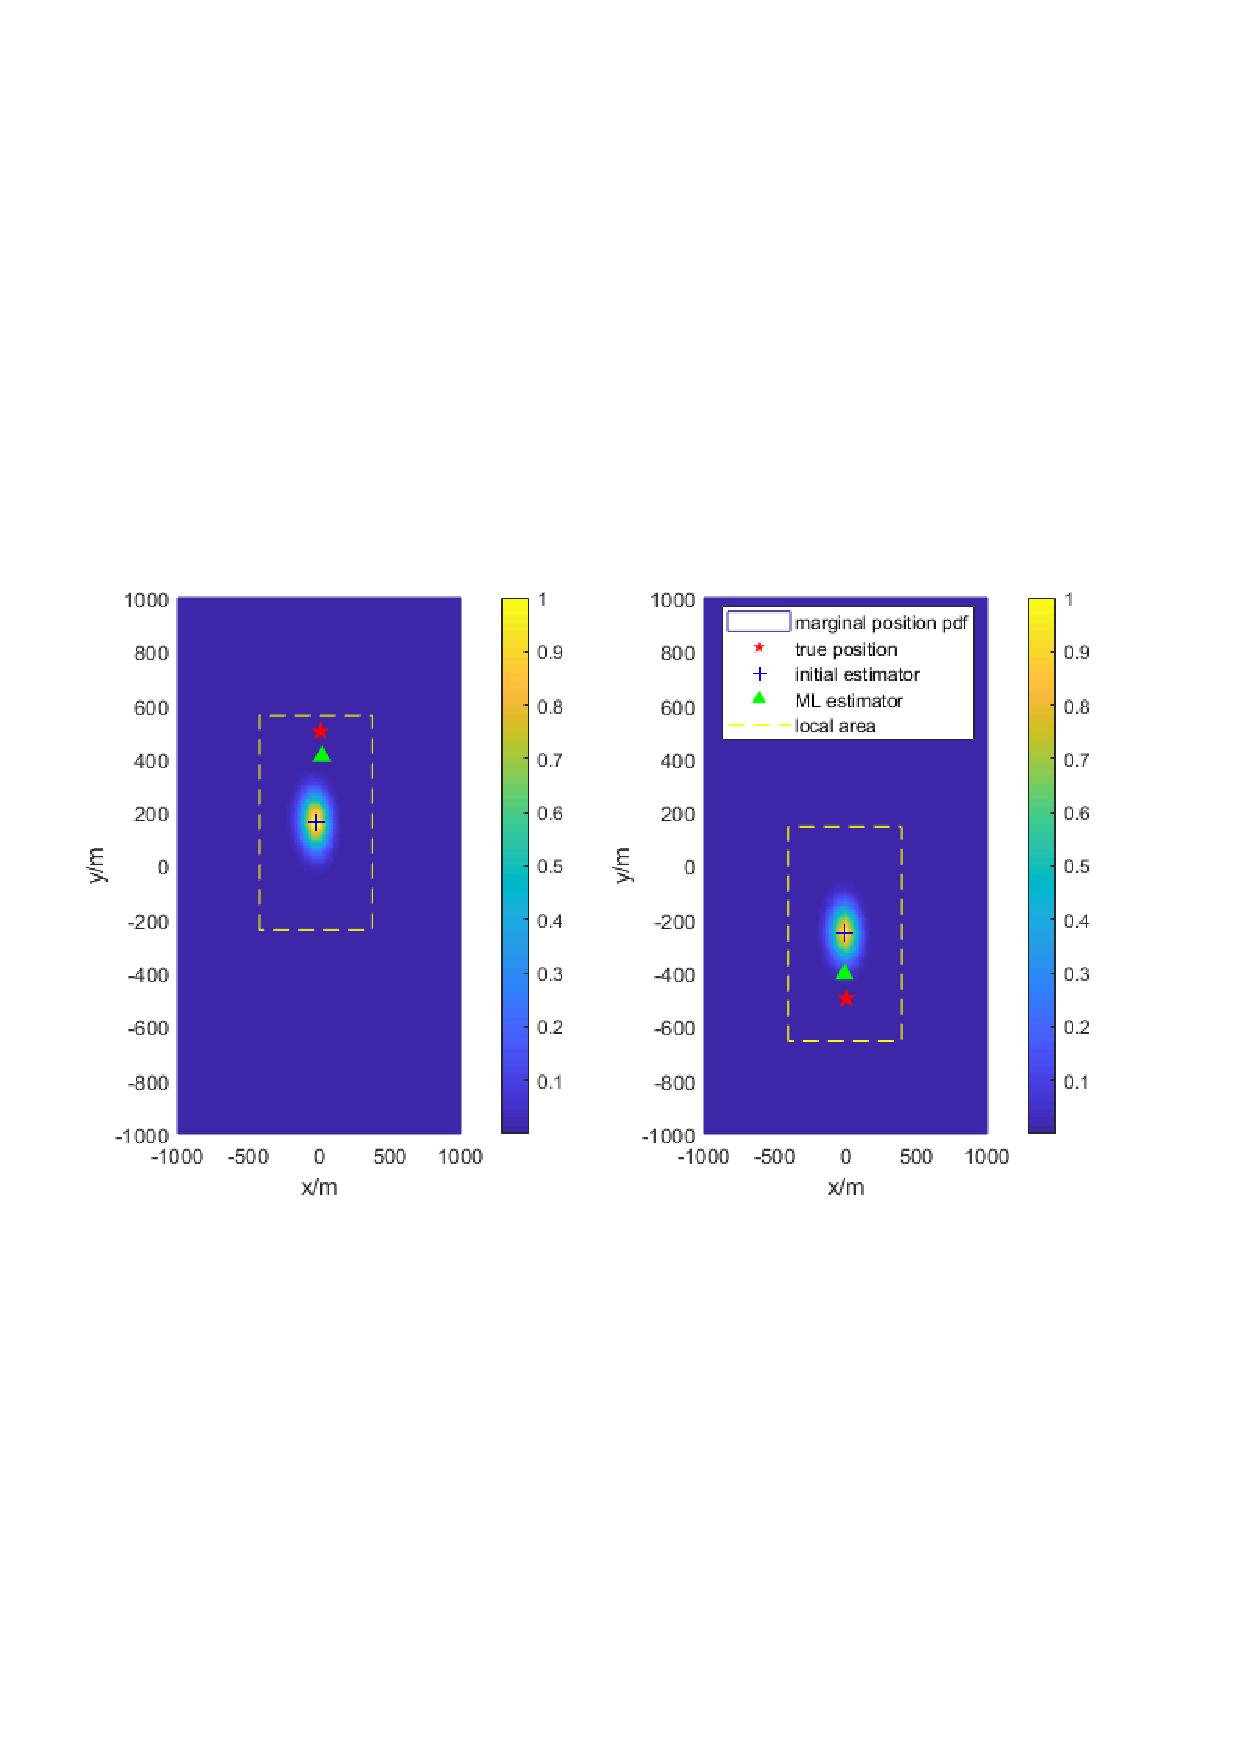
\includegraphics[width=1\textwidth]{pdfFigures/toolarge_rho1=500.pdf}}
    \centering
	\caption{the marginal position pdfs ($\rho_1=500$) of two adjacent emitters (the red solid pentacle) at $\boldsymbol{p}_1=(0,500)$m and $\boldsymbol{p}_2=(0,-500)$m respectively, the main simulation conditions are SNR=$15$dB, the number of sections $L=10$, the number of elements $M=3$, the bandwidth $B_w=20$kHz and the range $\Delta_x=\Delta_y=400$m (the yellow dotted rectangle).}\label{fig1}
\end{figure}

\begin{figure}[!t]
    \centerline{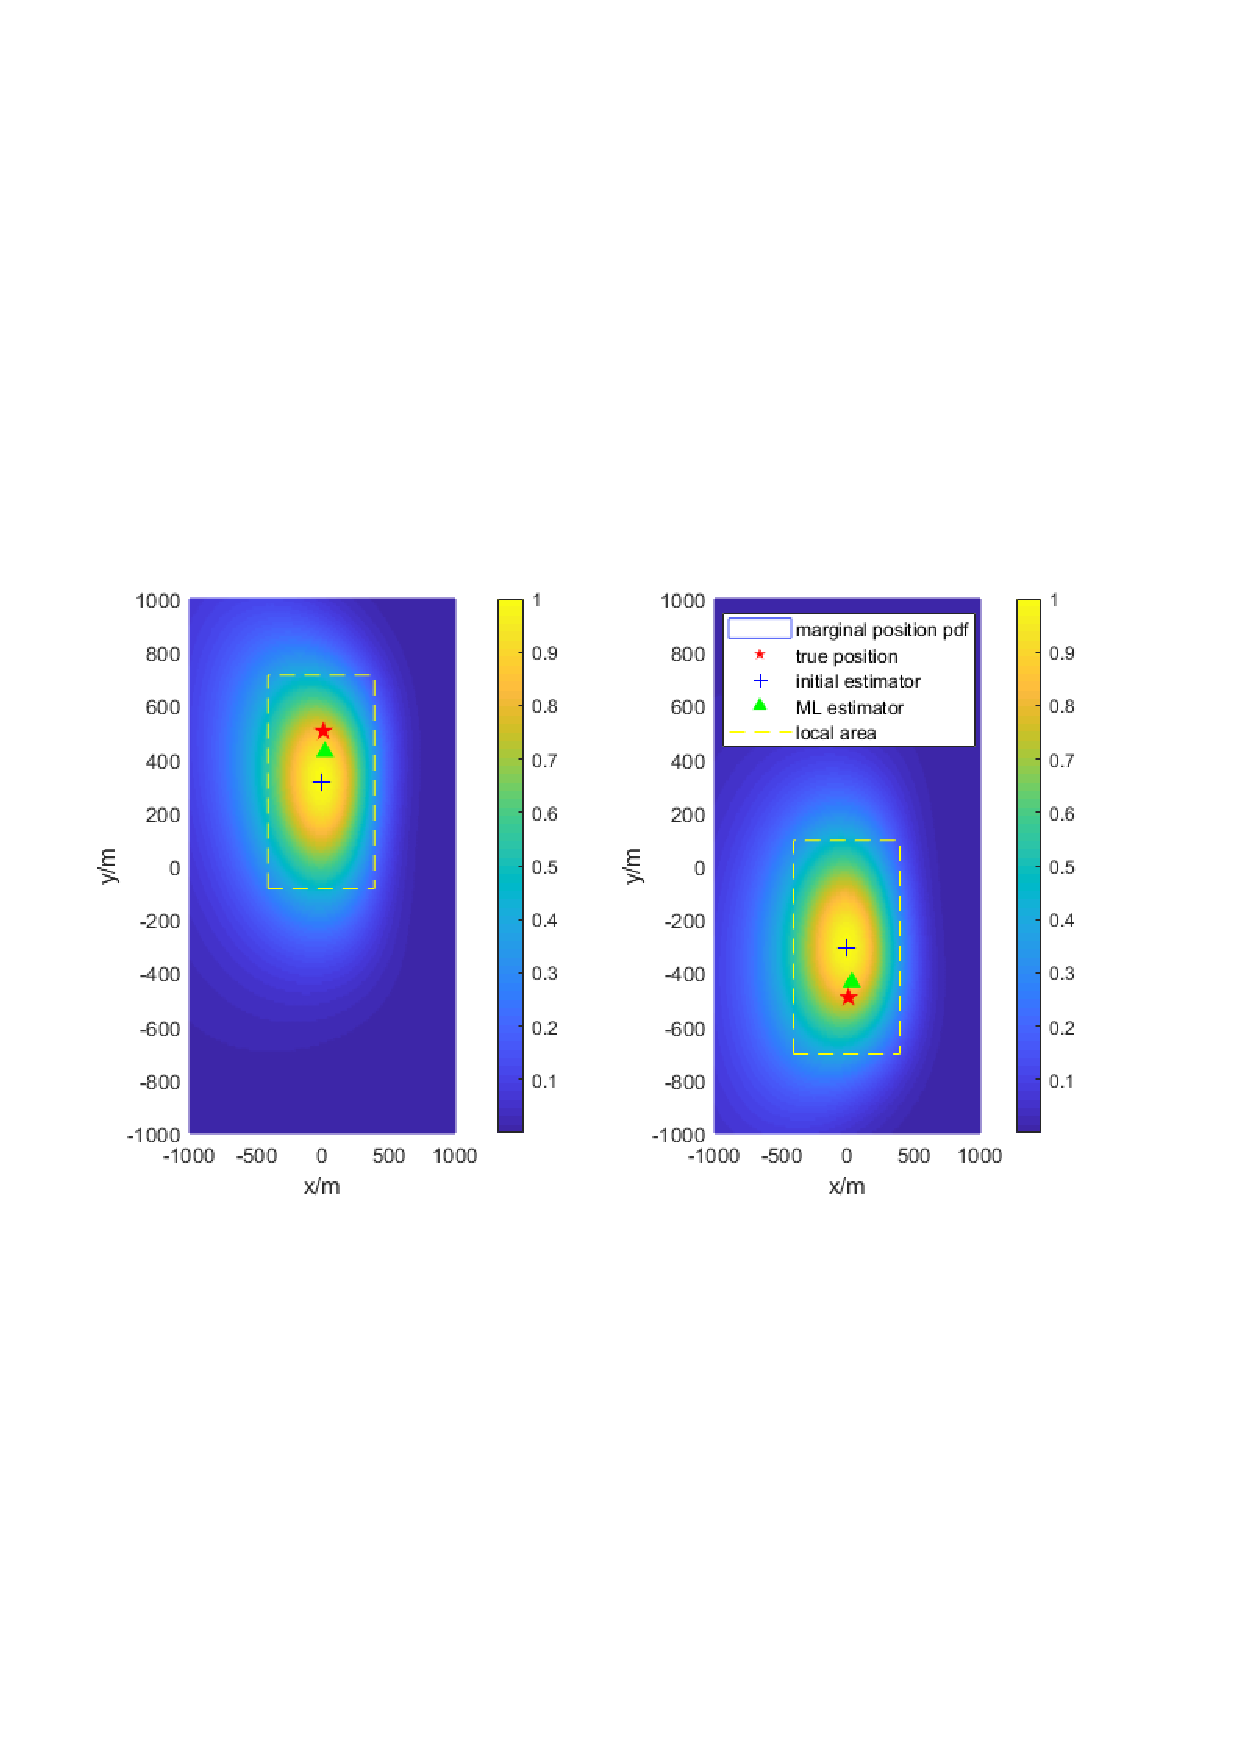
\includegraphics[width=1\textwidth]{pdfFigures/appropriate_rho1=20.pdf}}
    \centering
	\caption{the marginal position pdfs with appropriate $\rho_1=20$. Other conditions are the same.}\label{fig2}
\end{figure}

There is another detail about the super-parameters $\rho_1$ and $\rho_2$ to be stated. The distribution of probability mass in the local area $D_{\mathring{x}_q}\times D_{\mathring{y}_q}$ (or $D_{\mathring{t}_q}$) is governed by the super-parameter $\rho_1$ in the marginal position pdf $g_{\boldsymbol{p}}^{\text{mar}}(x_q,y_q)$ (or $\rho_2$ in the conditional transmitted time pdf $g_{\mathring{t}}^{\text{con}}(\mathring{t}_q\vert \boldsymbol{p}_q^{(r)})$) . Similarly to \eqref{gc}, the probability mass of $g_{\boldsymbol{p}}^{\text{mar}}(x_q,y_q)$ (or $g_{\mathring{t}}^{\text{con}}(\mathring{t}_q\vert \boldsymbol{p}_q^{(r)})$) would concentrate at the location of the maximum peak $(\mathring{x}_q,\mathring{y}_q)$ (or $\mathring{t}_q$) as $\rho_1$ (or $\rho_2$) increases. The too large $\rho_1$ (or $\rho_2$) would result in that the points, included in local area but far away from the maximum peak point, are hardly to be sampled (as seen in Fig.\ref{fig1}). The range parameter $\Delta_x$, $\Delta_y$ (or $\Delta_{\mathring{t}}$) and $\rho_1$ (or $\rho_2$) should, therefore, be well matched, in order to generate the required realizations efficiently (as seen in Fig.\ref{fig2}). 

\section{Complexity analysis}
The main computation of IS-based ML DPD algorithm concentrates on the generation of the required realizations and the computation of the IWs. The generation process involves evaluating the marginal position pdf $g_{\boldsymbol{p}}^{\text{mar}}(x_q,y_q)$ and the conditional transmitted time pdf $g_{\mathring{t}}^{\text{con}}(\mathring{t}_q \vert \boldsymbol{p}_q)$ at grids with different ranges and steps. The computational complexity, therefore, relies on the complexity of the two pdfs and the number of grid points. According to the definition of $g_{\boldsymbol{p}}^{\text{mar}}(x_q,y_q)$ \eqref{gpq}, its complexity is $\mathcal{O}(N^3)$ for the operation $\lambda_{\text{max}}$ involves the eigen-decomposition. The marginal position pdf $g_{\boldsymbol{p}}^{\text{mar}}(x_q,y_q)$ is evaluated in \eqref{step1}, \eqref{step5} and \eqref{step9}, at  $IJ$, $I'J'$ and $RJ'$ grid points respectively. The complexity of generating $Q$ groups of $\lbrace(\boldsymbol{p}_q^{(r)})\rbrace_{r=1}^{R},q=1,...,Q$ is, therefore, about $\mathcal{O}(Q(IJ+I'J'+RJ')N^3)$. Considering the $(q,r)$th matrix $\boldsymbol{\Pi}_q(\boldsymbol{p}_q^{(r)})$ in the marginal position pdf $g_{\boldsymbol{p}}^{\text{mar}}(x_q^{(r)},y_q^{(r)})$ is used in the conditional transmitted time pdf $g_{\mathring{t}}^{\text{con}}(\mathring{t}_q \vert \boldsymbol{p}_q^{(r)})$ again. The residual complexity of $g_{\mathring{t}}^{\text{con}}(\mathring{t}_q \vert \mathring{\boldsymbol{p}}_q^{(r)})$ is $\mathcal{O}(N^2)$. $g_{\mathring{t}}^{\text{con}}(\mathring{t}_q \vert \mathring{\boldsymbol{p}}_q^{(r)})$ is evaluated in \eqref{step3} and \eqref{step11}, at $S$ and $RS'$ grid points respectively. Therefore, the complexity of generating $Q$ groups of $\lbrace(\mathring{t}_q^{(r)})\rbrace_{r=1}^{R},q=1,...,Q$ is about $\mathcal{O}(Q(S+RS')N^2)$. According to the definition \eqref{SForm} and \eqref{gppt}, the values of $ \mathcal{G}(\boldsymbol{P},\mathring{\boldsymbol{t}})$ at all $R$ groups of realizations $\lbrace \boldsymbol{P}^{(r)},\mathring{\boldsymbol{t}}^{(r)}\rbrace_{r=1}^R$ have already been computed during the generation of realizations. Thus, the computation of IWs only involves $\mathcal{F}(\boldsymbol{P}^{(r)},\mathring{\boldsymbol{t}}^{(r)}),r=1,...,R$, of which the complexity is about $\mathcal{O}(RQ(LNMN_r+Q^2))$. In conclusion, the total complexity of IS-based ML DPD is about $\mathcal{O}(Q(G_{\boldsymbol{p}}N^3+(G_{\mathring{t}}+RN_r)N^2+RQ^2))$ where $G_{\boldsymbol{p}}=IJ+I'J'+RJ'$ and $G_{\mathring{t}}=S+RS'$.

\section{Numerical Simulation and Discussion}
\begin{figure}[!t]
    \centerline{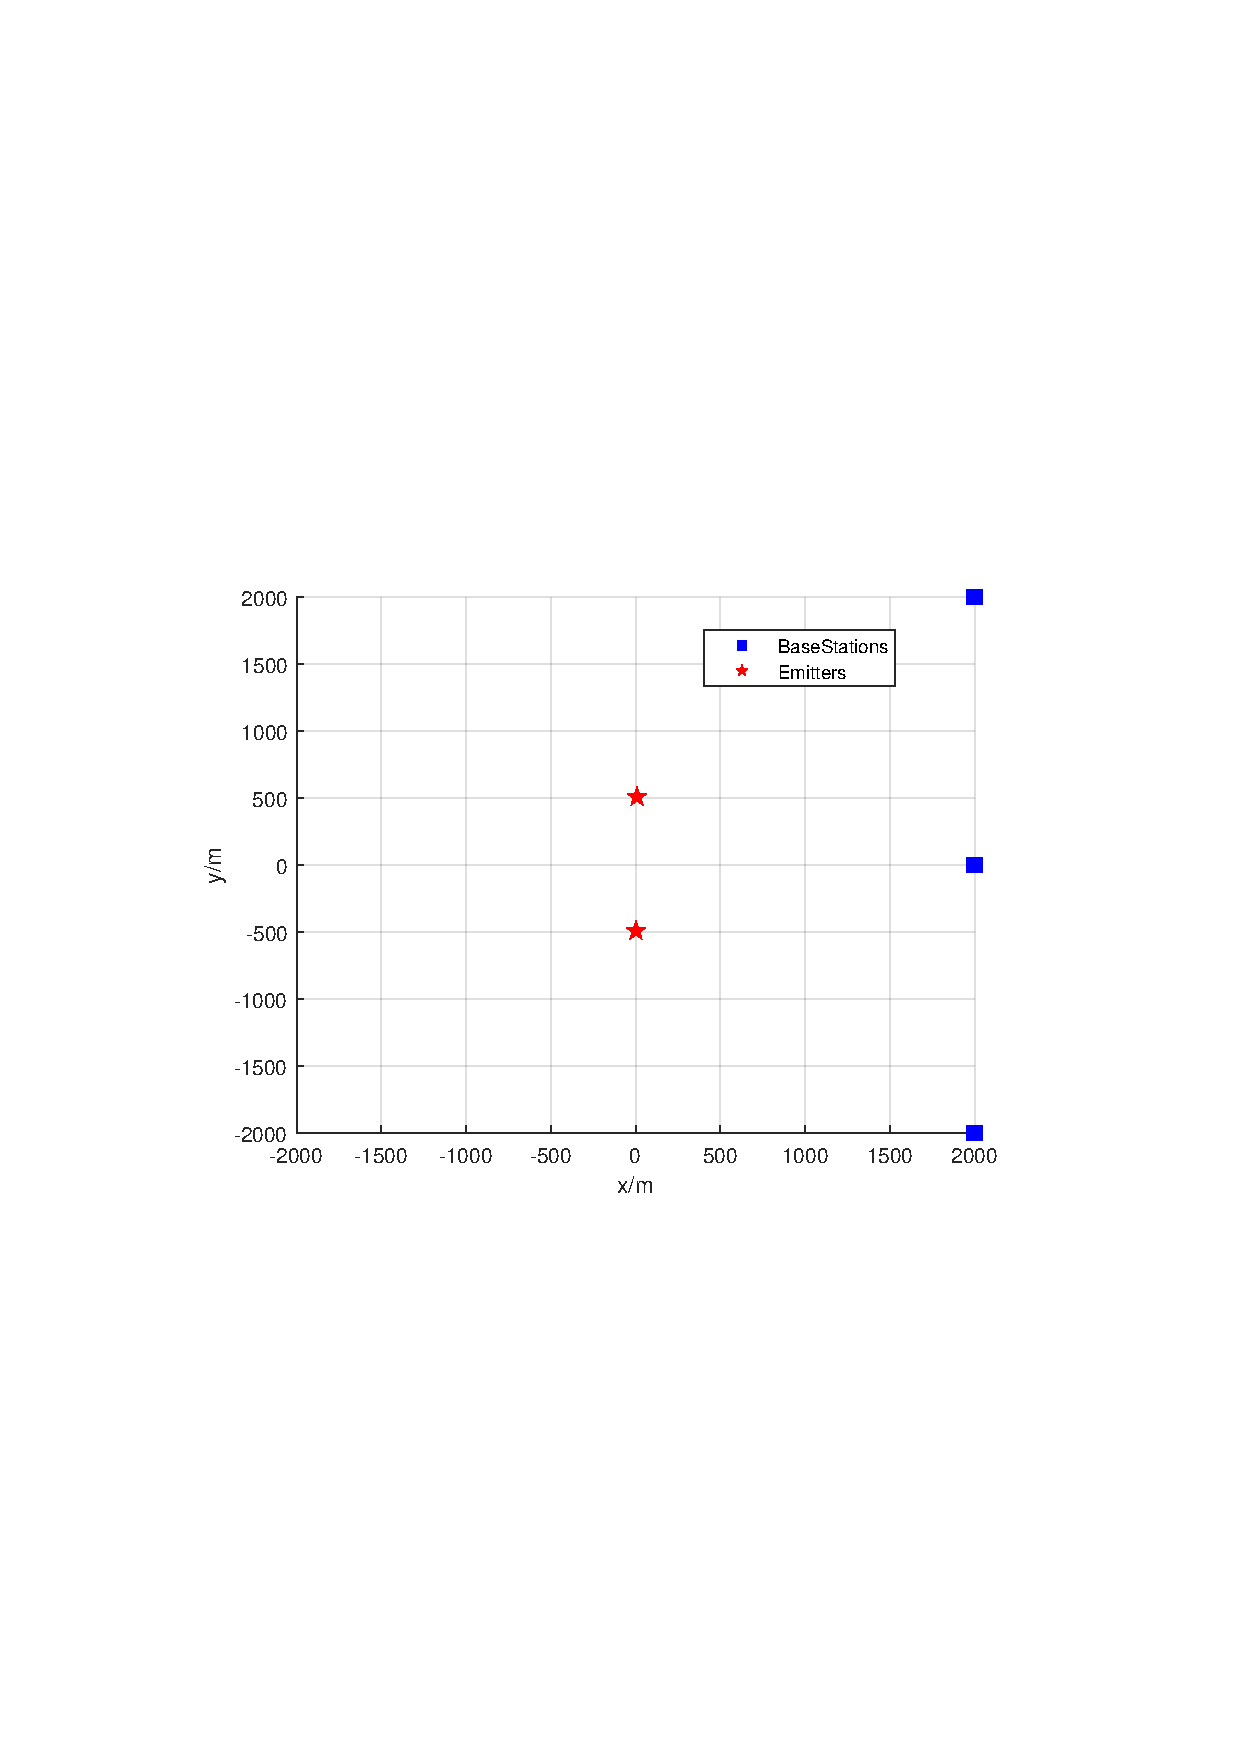
\includegraphics[width=1\textwidth]{pdfFigures/Senario.pdf}}
    \centering
	\caption{the simulation scenario}\label{fig3}
\end{figure}

\begin{figure}[!t]
    \centerline{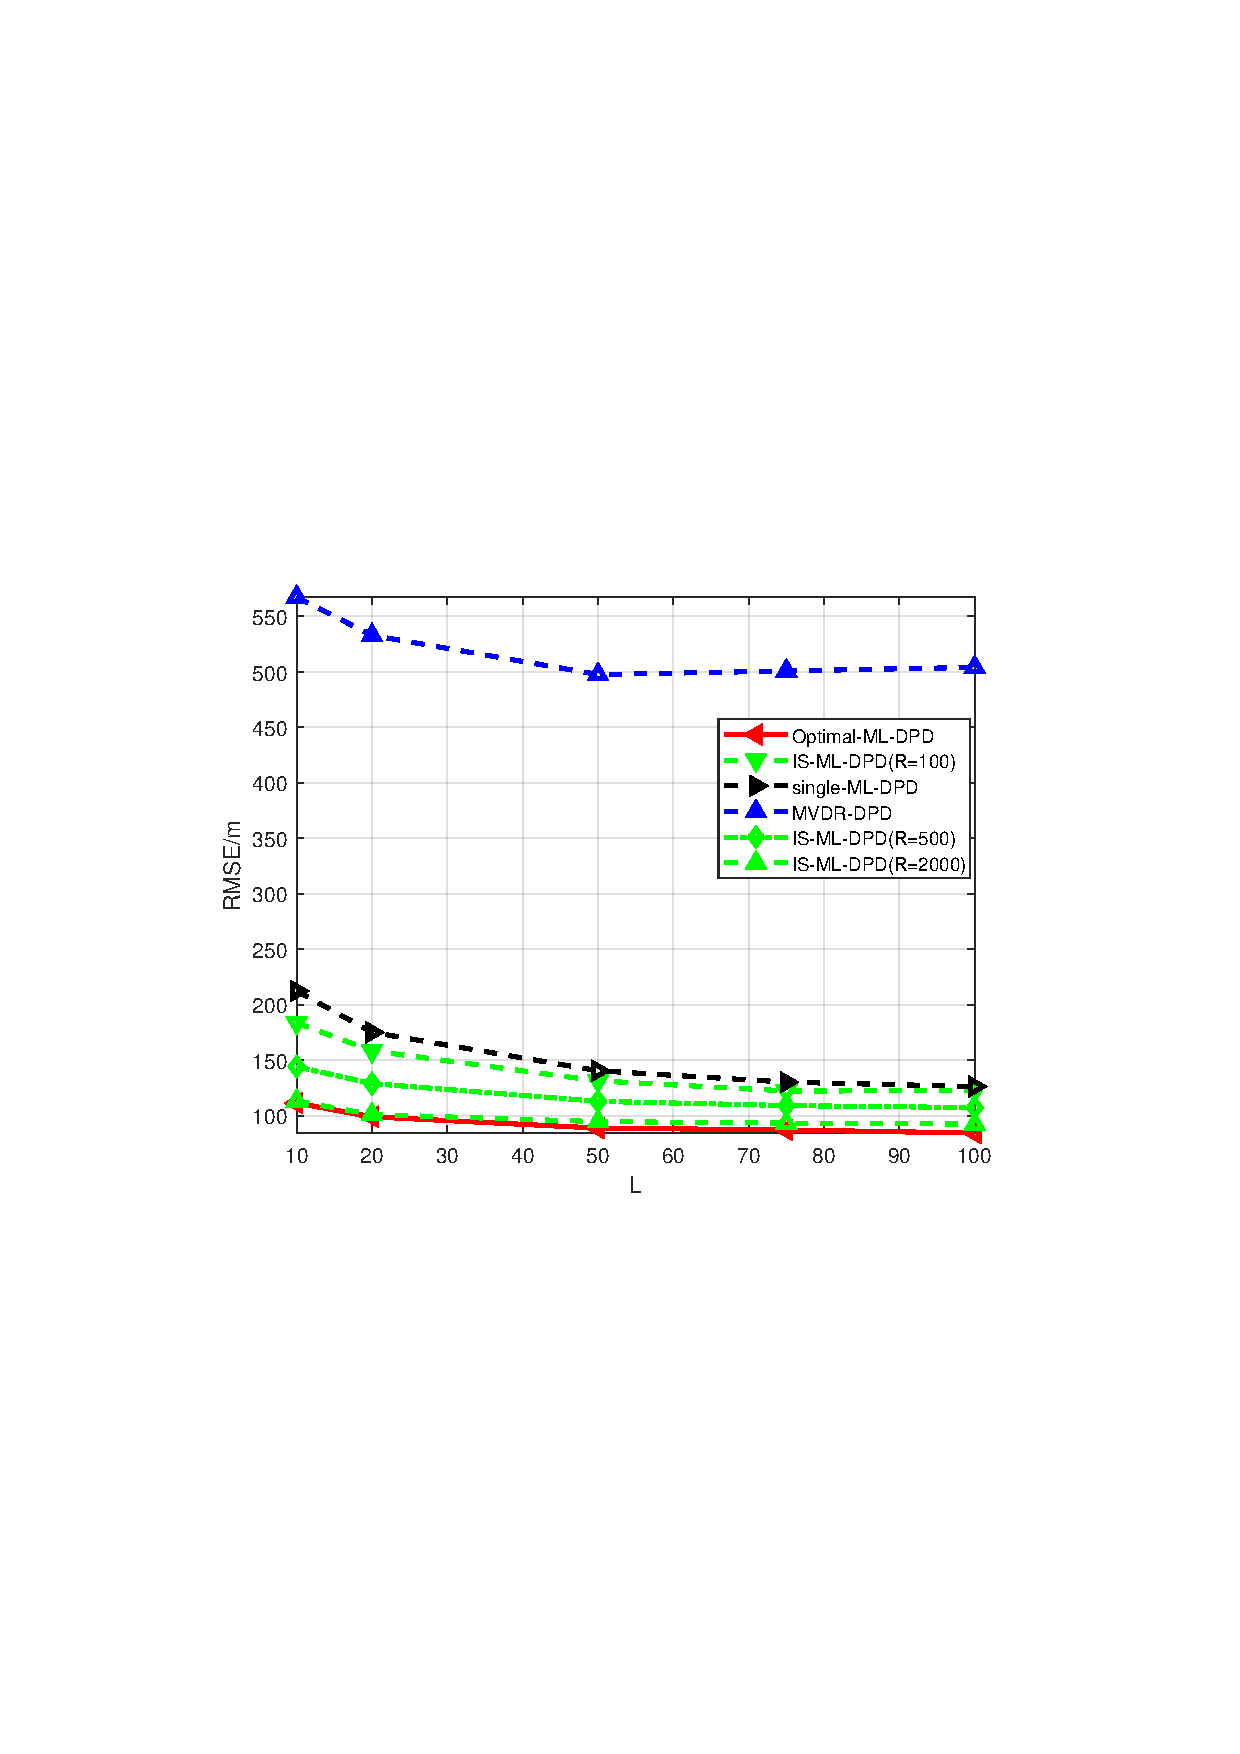
\includegraphics[width=1\textwidth]{pdfFigures/QvsRMSE(opt-IS(R100-500-2000)-SML-MVDR(1))SNR5dB.pdf}}
    \centering
	\caption{the RMSE of each estimator varies with the number of sections $L$. The signal bandwidth is $20$kHz and the $SNR=5$dB.}\label{fig4}
\end{figure}

\begin{figure}[!t]
    \centerline{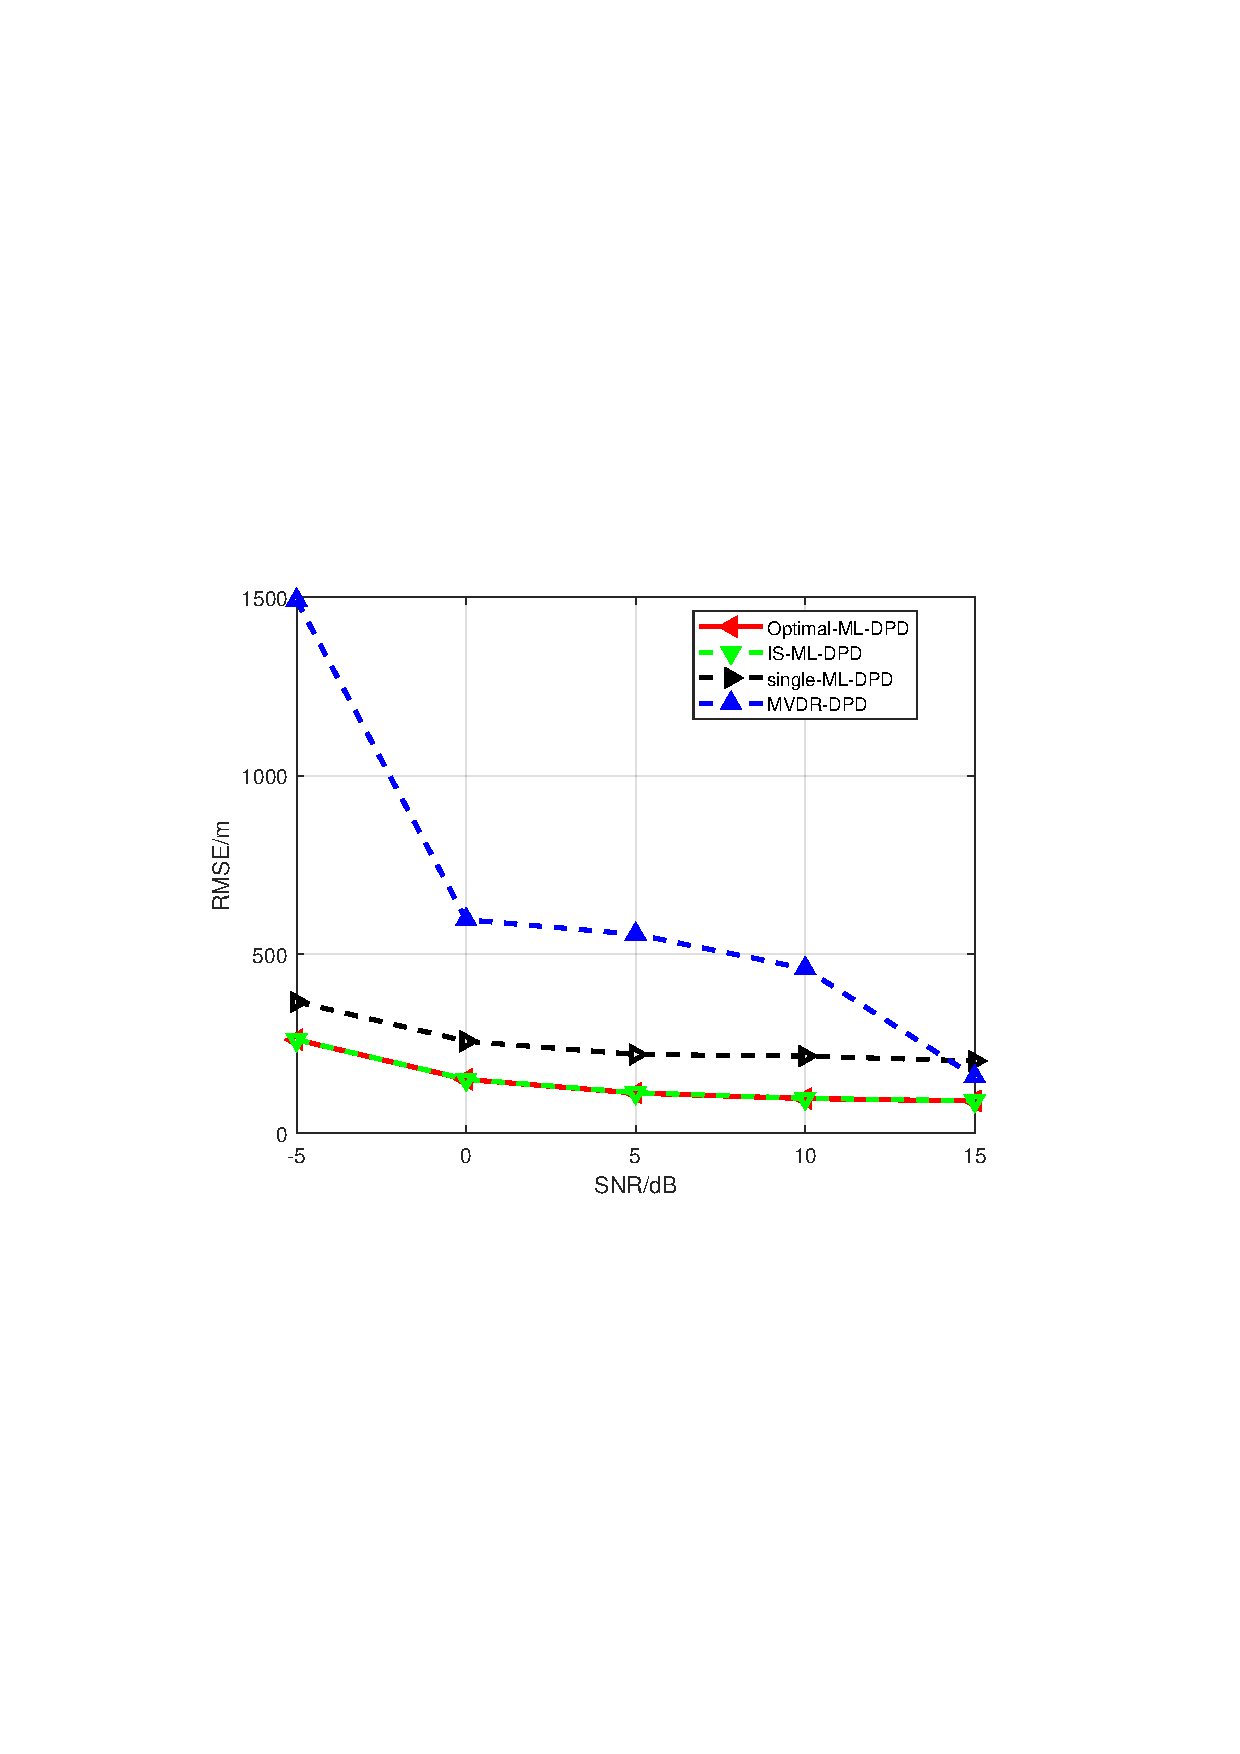
\includegraphics[width=1\textwidth]{pdfFigures/SNRvsRMSE(opt-IS(2000)-SML-MVDR(1))L10.pdf}}
    \centering
	\caption{the RMSE of each estimator varies with the SNR. The signal bandwidth is $20$kHz and the number of signal sections is $L=10$}\label{fig5}
\end{figure}

\begin{figure}[!t]
    \centerline{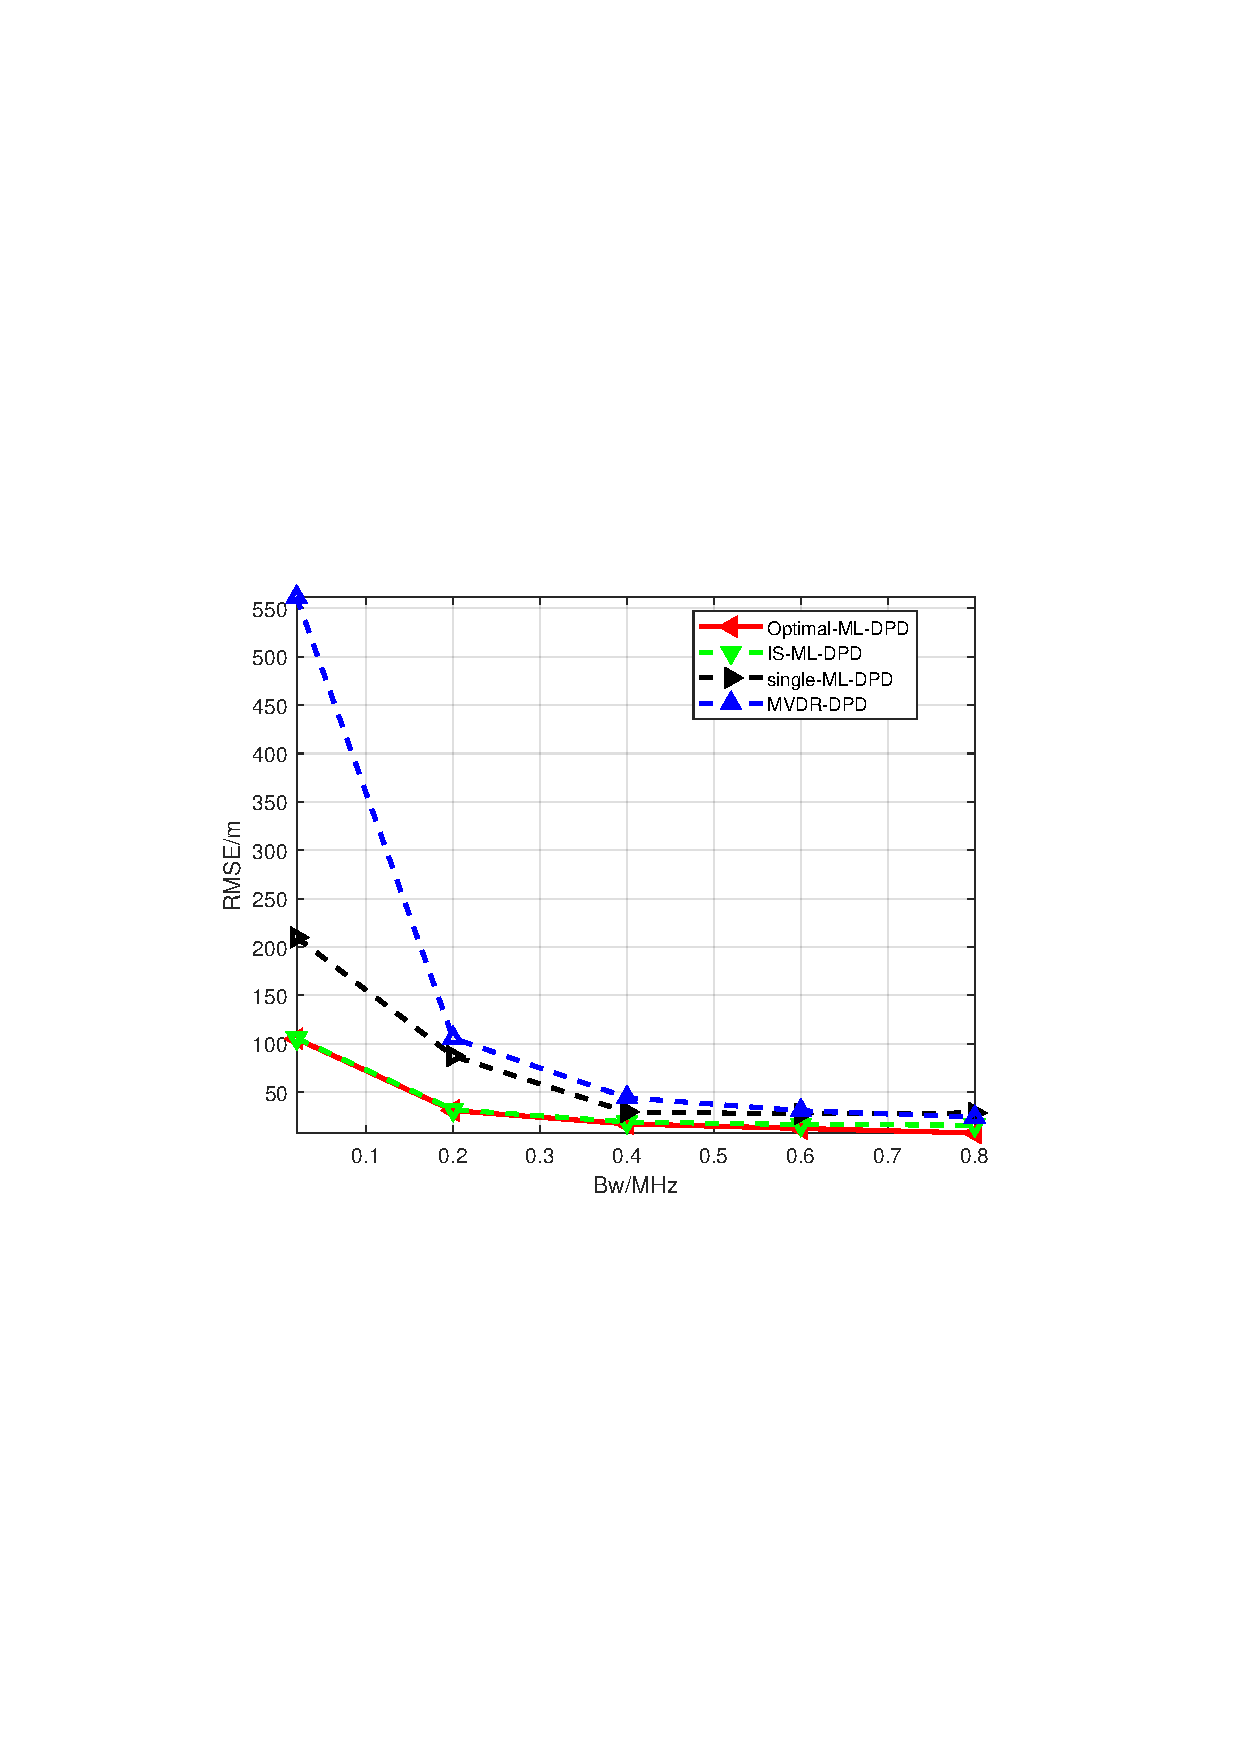
\includegraphics[width=1\textwidth]{pdfFigures/BWvsRMSE(snr5dBL10).pdf}}
    \centering
	\caption{the RMSE of each estimator varies with the bandwidth.}\label{fig6}
\end{figure}
In this section, we design several numerical simulations to evaluate the performance of the proposed IS based ML DPD estimator, denoted by IS-ML-DPD, and compare it with the decoupled ML DPD estimator proposed in \cite{DPD2005} and the MVDR based DPD estimator proposed in \cite{Tirer2015High}, denoted by single-ML-DPD and MVDR-DPD respectively. To give an explicit comparison with the exact ML estimator \eqref{MLE}, we also give its performance curve that are obtained by an iterative local optimization method using the true emitters' positions as the initial point, denoted by optimal-ML-DPD.

The single-ML-DPD in \cite{DPD2005} decouples the $Q(D+1)$-dimensional optimization problem into $Q$ independent $(D+1)$-dimensional optimization problems by approximating the emitters' correlation matrix  using a diagonal matrix (similar to the equation \eqref{GammaDiag}) under the assumption $L\to \infty$. The off-diagonal elements of the normalized correlation matrix \eqref{off-diagonal} tend to zero as the number of sections $L\to \infty$ since the transmitted signals among emitters are uncorrelated. The approximation in \cite{DPD2005}, consequently, may become inaccurate when the number of sections is limited in practice, which badly worsen the performance of single-ML-DPD estimator. 

According to the multiplier effect, The off-diagonal elements \eqref{off-diagonal} can also tend to zero as the DOA or TOA correlation coefficient $r_{doa,j}^{(u,v)}, r_{toa,j}^{(u,v)}\to 0$, even though the number of sections is limited in practice. It means that some estimators with high resolution, like the MVDR filter, may acquire better performance. The MVDR-DPD in \cite{Tirer2015High} constructs the MVDR filter on the location domain directly. It is well known that the MVDR principle requires the Distortionless Response (DR) vector \eqref{gamma} keeps the same among data samples (i.e., the signal sections), which means that the prior waveform information $s_q(n,l)$ has to be eliminated from the DR vector \eqref{gamma}. The MVDR-DPD estimator can, therefore, only use the DOA and TOA information to distinguish emitters. 

We use the Root Mean Square Error (RMSE) of the emitter's location estimation to evaluate the performance of each algorithm,
\begin{align}
    \text{RMSE}=\sqrt{\frac{\sum_{w=1}^W \Vert \boldsymbol{p}_1^{(w)}-\boldsymbol{p}_1\Vert ^2}{W}}
\end{align}
where the $W$ is the number of Monte Carlo simulations and we use $W=300$ to obtain the statistic results. 
As illustrated in Fig.\ref{fig3}, we consider the scenario where there are $N_r=3$ Base Stations (BS) at $(2,2)$km, $(2,0)$km and $(2,-2)$km respectively and $Q=2$ adjacent emitters at $\boldsymbol{p}_1=(0,500)$m and $\boldsymbol{p}_2=(0,-500)$m. Each BS is equipped with an Uniform Linear Array (ULA) of $M=3$ elements. The signals transmitted by the two emitters are two independent Gaussian random process. The Fourier coefficients of the transmitted signals are, consequently, complex Gaussian RVs, $s_q(n,l)\sim \mathcal{N}(0,\frac{10^{(SNR/10)}}{\sigma^2})$. The signal bandwidth is $20$kHz. The number of sections $L=10$ and the number of samples in each section is $N=5$. The transmitted time $\mathring{t}_q$ is selected from a Uniform Distribution $U[0,100\mu s]$.

The super-parameter $\rho_0=666$ in IW expressions \eqref{IWw} is set as large as possible while $\rho_1=20$ and $\rho_2=8$ are designed appropriately to make the ML solutions $\hat{\boldsymbol{p}}_q$ and $\hat{\mathring{t}}_q$ included in the main lobe of $g_{\boldsymbol{p}}^{\text{mar}}(x_q,y_q)$ and $g_{\mathring{t}}^{\text{con}}(\mathring{t}_q\vert \mathring{\boldsymbol{p}}_q)$ respectively. Corresponding to the size of the main lobe, the range parameters are set as $\Delta_x=\Delta_y=400$m and $\Delta_{\mathring{t}}=10\mu s$. These super-parameter values can be,statistically, acquired by plenty of simulations.

Note that the correlation coefficient $r_{sig}$ in \eqref{off-diagonal} would decrease until zero (the correlation information can be ignored) as the number of sections $L$ increases sufficiently, for the independence among $Q$ transmitted signals. Under the condition that $L$ is sufficiently large, the single-ML-DPD estimator would, therefore, achieve the performance of the optimal-ML-DPD estimator approximately. To indicate the IS-ML-DPD estimator's advantage when there are only a few signal sections, we start with varying the number of sections $L$ between $10$ and $100$ in the first simulation. Fig.\ref{fig4} shows that all three IS-ML-DPD performance curves (corresponding to the number of realizations $R=100,500$ and $2000$ respectively) locate in the gap between the performance curves of single-ML-DPD and optimal-ML-DPD. The localization accuracy of IS-ML-DPD improves as the number of realizations $R$ increases and approximates the accuracy of optimal-ML-DPD at $R=2000$. The reason is that enough realizations can guarantee that the realizations in vicinity of the ML solutions, with large IWs, can be sampled. It is worthy to note that $R=2000$ realizations is just a few in the $Q(D+1)=6$-dimensional parameter space. In another words, the complexity of brute searching for exact ML solution in $Q(D+1)=6$-dimensional parameter space is about $\mathcal{O}(N_g^{Q(D+1)})$ ($Ng$ is the number of grid points for each dimension), which is significantly larger than that of IS-ML-DPD. The MVDR-DPD estimator's RMSE is around half of the distance between the two emitters at all $L$ candidate values, which indicates that it fails to distinguish the two adjacent emitters at $SNR=5dB,Bw=20$kHz since the beforehand waveform information is not used at all.

Fig.\ref{fig5} shows that the RMSE of each algorithm varies with SNR in the second simulation. The SNR varies between $-5$dB and $15$dB. It can be seen that the IS-ML-DPD (The number of realizations $R=2000$) also approximates the performance of the optimal-ML-DPD at all SNR. The reason why there is a performance gap between single-ML-DPD and the IS-ML-DPD (or the optimal-ML-DPD) is that there exists the correlation among emitters for the limited observation resources ($B_w=20$kHz,$L=10$), which results in the interferences with one another. In such case, assuming the independence among emitters to decouple the multidimensional optimization problem is sub-optimal. On the condition of limited observation resources, the MVDR-DPD estimator is also unable to distinguish the two adjacent emitters until $SNR= 15$dB. The MVDR-DPD shows the higher resolution than single-ML-DPD and approximates the accuracy of IS-ML-DPD at relatively high SNR.

The first two simulations indicate that the single-ML-DPD and MVDR-DPD are sub-optimal while the IS-ML-DPD is able to approximate the performance of the optimal-ML-DPD in the case of limited observation resources. To further validate this result, we gradually increase the signal bandwidth $B_w$ from $20$kHz to $800$kHz in the third simulation. As expected, the IS-ML-DPD outperforms the single-ML-DPD and MVDR-DPD, approximating the performance of the optimal-ML-DPD, when $B_w\leq400$kHz and all estimators' performances converge together as the $B_w$ increases.

\appendix
\section{The derivation of SLF}\label{ApA}
Our derivation starts with a vector definition as follows,
\begin{align}\label{gammaqjl}
    \boldsymbol{\gamma}_{q,j,l}\triangleq\boldsymbol{\Phi}_{q,j,l}(\boldsymbol{p}_q)\boldsymbol{b}(\mathring{t}_q)
\end{align}
where
\begin{align}\label{Phi}
    \boldsymbol{\Phi}_{q,j,l}(\boldsymbol{p}_q)&\triangleq\boldsymbol{\Lambda}_j(\boldsymbol{p}_q,s_q(l))\otimes \boldsymbol{a}_j(\boldsymbol{p}_q)\\
    \boldsymbol{b}(\mathring{t}_q)&\triangleq[e^{-j2\pi f_1\mathring{t}_q},...,e^{-j2\pi f_N\mathring{t}_q}]^T\\
    \boldsymbol{\Lambda}_j(\boldsymbol{p}_q,s_q(l))&\triangleq 
    \left[ 
    \begin{array}{ccc}
        s_q(1,l)e^{-j2\pi f_1\tau_j(\boldsymbol{p}_q)}& \ldots & 0\\
        \vdots&\ddots&\vdots\\
        0&\ldots&s_q(N,l)e^{-j2\pi f_N\tau_j(\boldsymbol{p}_q)}
    \end{array}
    \right ]   
\end{align}
substituting \eqref{gammaqjl} and \eqref{Phi} into \eqref{glc}, we get
\begin{align}
    \tilde{\ell}_c(\boldsymbol{p}_q,\mathring{t}_q)&= \sum_{j=1}^{N_r} \sum_{l=1}^{L} \boldsymbol{\gamma}_{q,j,l}^H\boldsymbol{y}_j(l)\boldsymbol{y}_j^H(l)\boldsymbol{\gamma}_{q,j,l}\\
    &=\boldsymbol{b}^H(\mathring{t}_q)\underbrace{\left(\sum_{j=1}^{N_r} \sum_{l=1}^{L} \boldsymbol{\Phi}^H_{q,j,l}(\boldsymbol{p}_q)\boldsymbol{y}_j(l)\boldsymbol{y}_j^H(l)\boldsymbol{\Phi}_{q,j,l}(\boldsymbol{p}_q)\right)}_{\triangleq\boldsymbol{\Pi}_q(\boldsymbol{p}_q)} \boldsymbol{b}(\mathring{t}_q)
\end{align}
The right hand of the second equation is a non-normalized Rayleigh Quotient with respect to $\mathring{t}_q$. Consequently, maximizing $\tilde{\ell}_c(\boldsymbol{p}_q,\mathring{t}_q)$ with respect to $\mathring{t}_q$, we get,
\begin{align}\label{ell_lambda}
    \ell_q(\boldsymbol{p}_q)\triangleq\lambda_{\text{max}}(\boldsymbol{\Pi}_q(\boldsymbol{p}_q))
\end{align}
where the notation $\lambda_{\text{max}}(\boldsymbol{X})$ denotes the maximum eigenvalue of the matrix $\boldsymbol{X}$. Substituting \eqref{ell_lambda} into \eqref{gmar}, we get the marginal pdf of the $q$th emitter's position,
\begin{align}\label{gpq}
    g_{\boldsymbol{p}}^{\text{mar}}(\boldsymbol{p}_q)=\frac{e^{\rho_1\lambda_{\text{max}}(\boldsymbol{\Pi}_q(\boldsymbol{p}_q))}}{\int e^{\rho_1\lambda_{\text{max}}(\boldsymbol{\Pi}_q(\boldsymbol{p}_q))} d\boldsymbol{p}_q}
\end{align}

\section*{References}
\bibliography{mybibfile}

\end{document}